\documentclass[a4paper,twoside]{article}

\usepackage{epsfig}
\usepackage{subcaption}
\usepackage{calc}
\usepackage{amssymb}
\usepackage{amstext}
\usepackage{cite}
\usepackage{amsmath,amssymb,amsfonts}
\usepackage{apalike}
\usepackage{algorithm2e}
\usepackage{SCITEPRESS}
\usepackage{float}
\usepackage{graphicx,url}
\usepackage{balance}
\usepackage{booktabs}
\usepackage{color}
\usepackage{xcolor}
\definecolor{stronggreen}{RGB}{0,150,0}

\begin{document}

\title{Zero-Touch Selection of Virtual Network Embedding Algorithms using Multi-Objective Decision Trees}

\author{\authorname{Blind Review\sup{1}\orcidAuthor{0000-0000-0000-0000} and Blind Review\sup{1}\orcidAuthor{0000-0000-0000-0000}}
\affiliation{\sup{1}Blind Review}
\email{\{first\_author, second\_author\}@blind.review}
}

\keywords{
Virtual Network Embedding, Decision Trees, Multi-Objective Optimization, Zero-Touch Administration, Interpretable Machine Learning}

\abstract{
The \textit{Virtual Network Embedding} (VNE) problem is fundamental in cloud infrastructures where providers share physical resources among multiple tenants. Mapping virtual network requests onto the physical infrastructure, satisfying capacity constraints and optimizing objectives such as acceptance rate and resource consumption, is NP-hard, motivating the development of various algorithms ranging from exact methods based on Mixed Integer Programming (MIP) to heuristics and meta-heuristics. However, no algorithm presents superior performance in all scenarios. This work proposes an approach based on multi-objective decision trees to automatically select the most appropriate VNE algorithm for each request, considering the physical network state and request characteristics. The method employs three specialized models, each optimized for a specific objective (acceptance rate, revenue-cost ratio, and average revenue), allowing adaptation to operational priorities at runtime. Experimental validation on three datacenter topologies with 8,000 requests presents top-3 accuracy between 79.1\% and 85.9\% in predicting the best algorithm, with an improvement of +32.9 percentage points in acceptance rate compared to the fixed baseline algorithm. The approach offers interpretability through explicit decision paths, inference latency below 1\,ms enabling online operation, and autonomous operation capability aligned with zero-touch administration requirements.}

\onecolumn \maketitle \normalsize \setcounter{footnote}{0} \vfill

%===================================================================

\section{Introduction}
\label{sec:Intro}

The \textit{Virtual Network Embedding} (VNE) problem has emerged as an essential enabler for modern networks, including cloud datacenters, edge computing, and 5G networks, due to its flexibility and scalability. VNE has become critical in infrastructures where providers share physical network resources among multiple tenants. The problem addresses the challenge of mapping virtual network requests (VNRs) to the physical infrastructure, satisfying capacity constraints, and optimizing objectives such as acceptance rate, processing time, and energy consumption.
%
Over the past two decades, numerous VNE algorithms have been proposed, ranging from exact methods based on Mixed Integer Programming (MIP) to heuristics and meta-heuristics.
A fundamental challenge remains: \textit{no single algorithm presents consistently superior performance in all scenarios}.
Different VNR characteristics (size, topology, demands) and physical network states (utilization, resource fragmentation) require distinct policies.
%
Traditional VNE deployment approaches typically select a single algorithm for all requests, regardless of their characteristics or the current state of the network. This strategy does not take advantage of the strengths of different algorithms for specific workload scenarios.

Additionally, zero-touch administration of virtualized networks has become a critical requirement in modern infrastructures.
The concept of \textit{Zero-Touch Network and Service Management} (ZSM), formalized by the ETSI standard since 2017~\cite{etsi-zsm}, refers to the ability of systems to operate autonomously through programmable control mechanisms, virtualization, and closed-loop feedback, with minimal human intervention.
Industry research indicates that autonomous networks can significantly reduce operational costs.
However, the gap between research and deployment remains: while deep Reinforcement Learning (RL) and optimization systems achieve high performance, they lack interpretability and suffer from decision latency inadequate for real-time systems~\cite{white2024zerotough}.
Therefore, systems that perform automatic VNE algorithm selection without operator intervention are fundamental to achieving truly autonomous operation.

\textcolor{stronggreen}{In many computational domains, the problem of automatically selecting algorithms has been extensively studied~\cite{rice1976algorithm}, showing that different instances benefit from different methods and that portfolio-based selectors often outperform single fixed algorithms~\cite{xu2012satzilla}. Surveys on automated algorithm selection~\cite{kotthoff2012algorithm,kerschke2019comprehensive} and meta-learning~\cite{vanschoren2018meta} report that data-driven selectors and portfolio methods are effective at adapting to heterogeneous instances, but typically rely on complex or black-box models whose internal decision logic is hard to interpret. Recent knowledge-based schedulers for HPC data centers~\cite{koslowski2025knowledge-based} follow a similar philosophy, learning from historical scheduling decisions to combine existing policies and improve performance metrics such as bounded slowdown and waiting time. However, these approaches focus primarily on aggregate performance indicators and rarely provide explicit, human-readable rules that explain \textit{why} a particular algorithm or policy is selected under a given contextual state. In the context of Virtual Network Embedding and Zero-Touch administration, this lack of interpretability is a critical limitation~\cite{white2024zerotough}, since operators and regulators require auditable decision rules rather than opaque recommendations.}

\textcolor{stronggreen}{Against this background, this work can be seen as bringing together two lines of research: automatic algorithm selection and interpretable network automation. Similar to portfolio and knowledge-based schedulers, we learn from historical executions of existing VNE algorithms to build a selector that adapts to request characteristics and network state. At the same time, by using decision trees we obtain explicit decision paths that can be inspected, audited, and translated into natural-language rules. This combination directly addresses the gap in current automatic selection approaches, which improve performance but do not explain \textit{why} decisions are made, and aligns with ZSM requirements for transparent, accountable automation.}

In this context, the present work proposes an approach based on multi-objective decision trees to automatically select the most appropriate VNE algorithm for each request, considering the network state and request characteristics.
Unlike a single model, the method employs three specialized models, each optimized for a specific objective (acceptance rate, revenue-cost ratio, average revenue), allowing adaptation to operational priorities at runtime, with inference latency below 1\,ms enabling online operation.

This work is organized as follows: Section~\ref{sec:RefTeo} presents the theoretical background; Section~\ref{sec:RelatedWork} discusses related work; Section~\ref{sec:Proposal} describes the methodology; Section~\ref{sec:Results} presents experimental results; and Section~\ref{sec:Conclusion} presents conclusions.

\section{Background and Motivation}
\label{sec:RefTeo}

\subsection{Virtual Network Embedding}
\label{subsec:vne}

Virtual Network Embedding (VNE) is the process of mapping virtual network requests onto a shared physical network infrastructure~\cite{fischer2013vne-survey}.
A virtual network request $G_v = (N_v, L_v)$ consists of a set of virtual nodes $N_v$ and virtual links $L_v$, where each node and link has specific resource demands (CPU, memory, bandwidth).
The physical network $G_p = (N_p, L_p)$ provides the computational and network substrate.
%
The VNE problem can be decomposed into two subproblems: (i) mapping virtual nodes to physical nodes; and (ii) mapping virtual links to paths in the physical network. The objective is to maximize metrics such as VNR acceptance rate, minimize processing time, and optimize physical resource consumption.
%
The VNE problem is NP-hard~\cite{fischer2013vne-survey}, motivating the development of various algorithm classes:

\begin{itemize}
    \item Exact Algorithms: Methods such as Mixed Integer Programming (MIP) guarantee optimal solutions, but have exponential complexity.
    \item Heuristics: Greedy algorithms that make local decisions based on node \textit{rankings}, offering reduced execution time with variable solution quality.
    \item Meta-heuristics: Techniques such as genetic algorithms (GA), particle swarm optimization (PSO), and Monte Carlo tree search (MCTS) employ stochastic search that balances exploration and quality.
\end{itemize}

Given that different VNE algorithms present variable performance depending on context, a mechanism becomes necessary to automatically select the most appropriate algorithm. The next section presents decision trees as a machine learning technique suitable for this contextual selection.

\subsection{Decision Trees for Classification}
\label{subsec:trees}

Decision trees are supervised learning models that recursively partition the feature space to create homogeneous prediction regions.
The tree starts at a root node containing all training data.
Progressively, at each level, the tree subdivides the feature space using binary decisions, creating specialized branches.
Each leaf (terminal node) represents a final prediction, in this context, which VNE algorithm is most appropriate.



At each internal node, the tree selects a feature and a threshold, dividing data into two subsets. The splitting criterion uses Gini index or information gain, maximizing class isolation. Each path from root to leaf represents an interpretable decision rule.
%
Figure~\ref{fig:tree-example-path} illustrates an example of a decision path, showing how each intermediate decision in the tree progressively reduces the solution space until reaching a final recommendation by evaluating the current state of both the Physical Network (PN) and Virtual Network Request (VNR) through a series of decision nodes. The highlighted path (shown in green) illustrates a concrete example where the tree recommends the MIP algorithm. Starting from the root node containing all training data, the tree first evaluates whether the physical network's node utilization is below or equal to 60\%. Following the affirmative branch, the second decision examines whether the VNR size contains 5 nodes or fewer. For small-scale requests in low-utilization networks, a third decision evaluates whether node utilization exceeds 70\%, identifying a congestion-prone scenario. This specific combination of conditions leads to the recommendation of MIP (Mixed Integer Programming), an exact algorithm guaranteed to find optimal solutions in congestion scenarios. The extracted rule can be formalized as: \textit{IF} (node\_utilization $\leq$ 60\%) \textit{AND} (vnr\_size $\leq$ 5 nodes) \textit{AND} (node\_utilization $>$ 70\%) \textit{THEN} select MIP. This automated decision-making process eliminates the need for manual algorithm selection by encoding expert knowledge about when different VNE algorithms perform optimally based on measurable network and request characteristics.
%



\begin{figure*}[t]
    \centering
    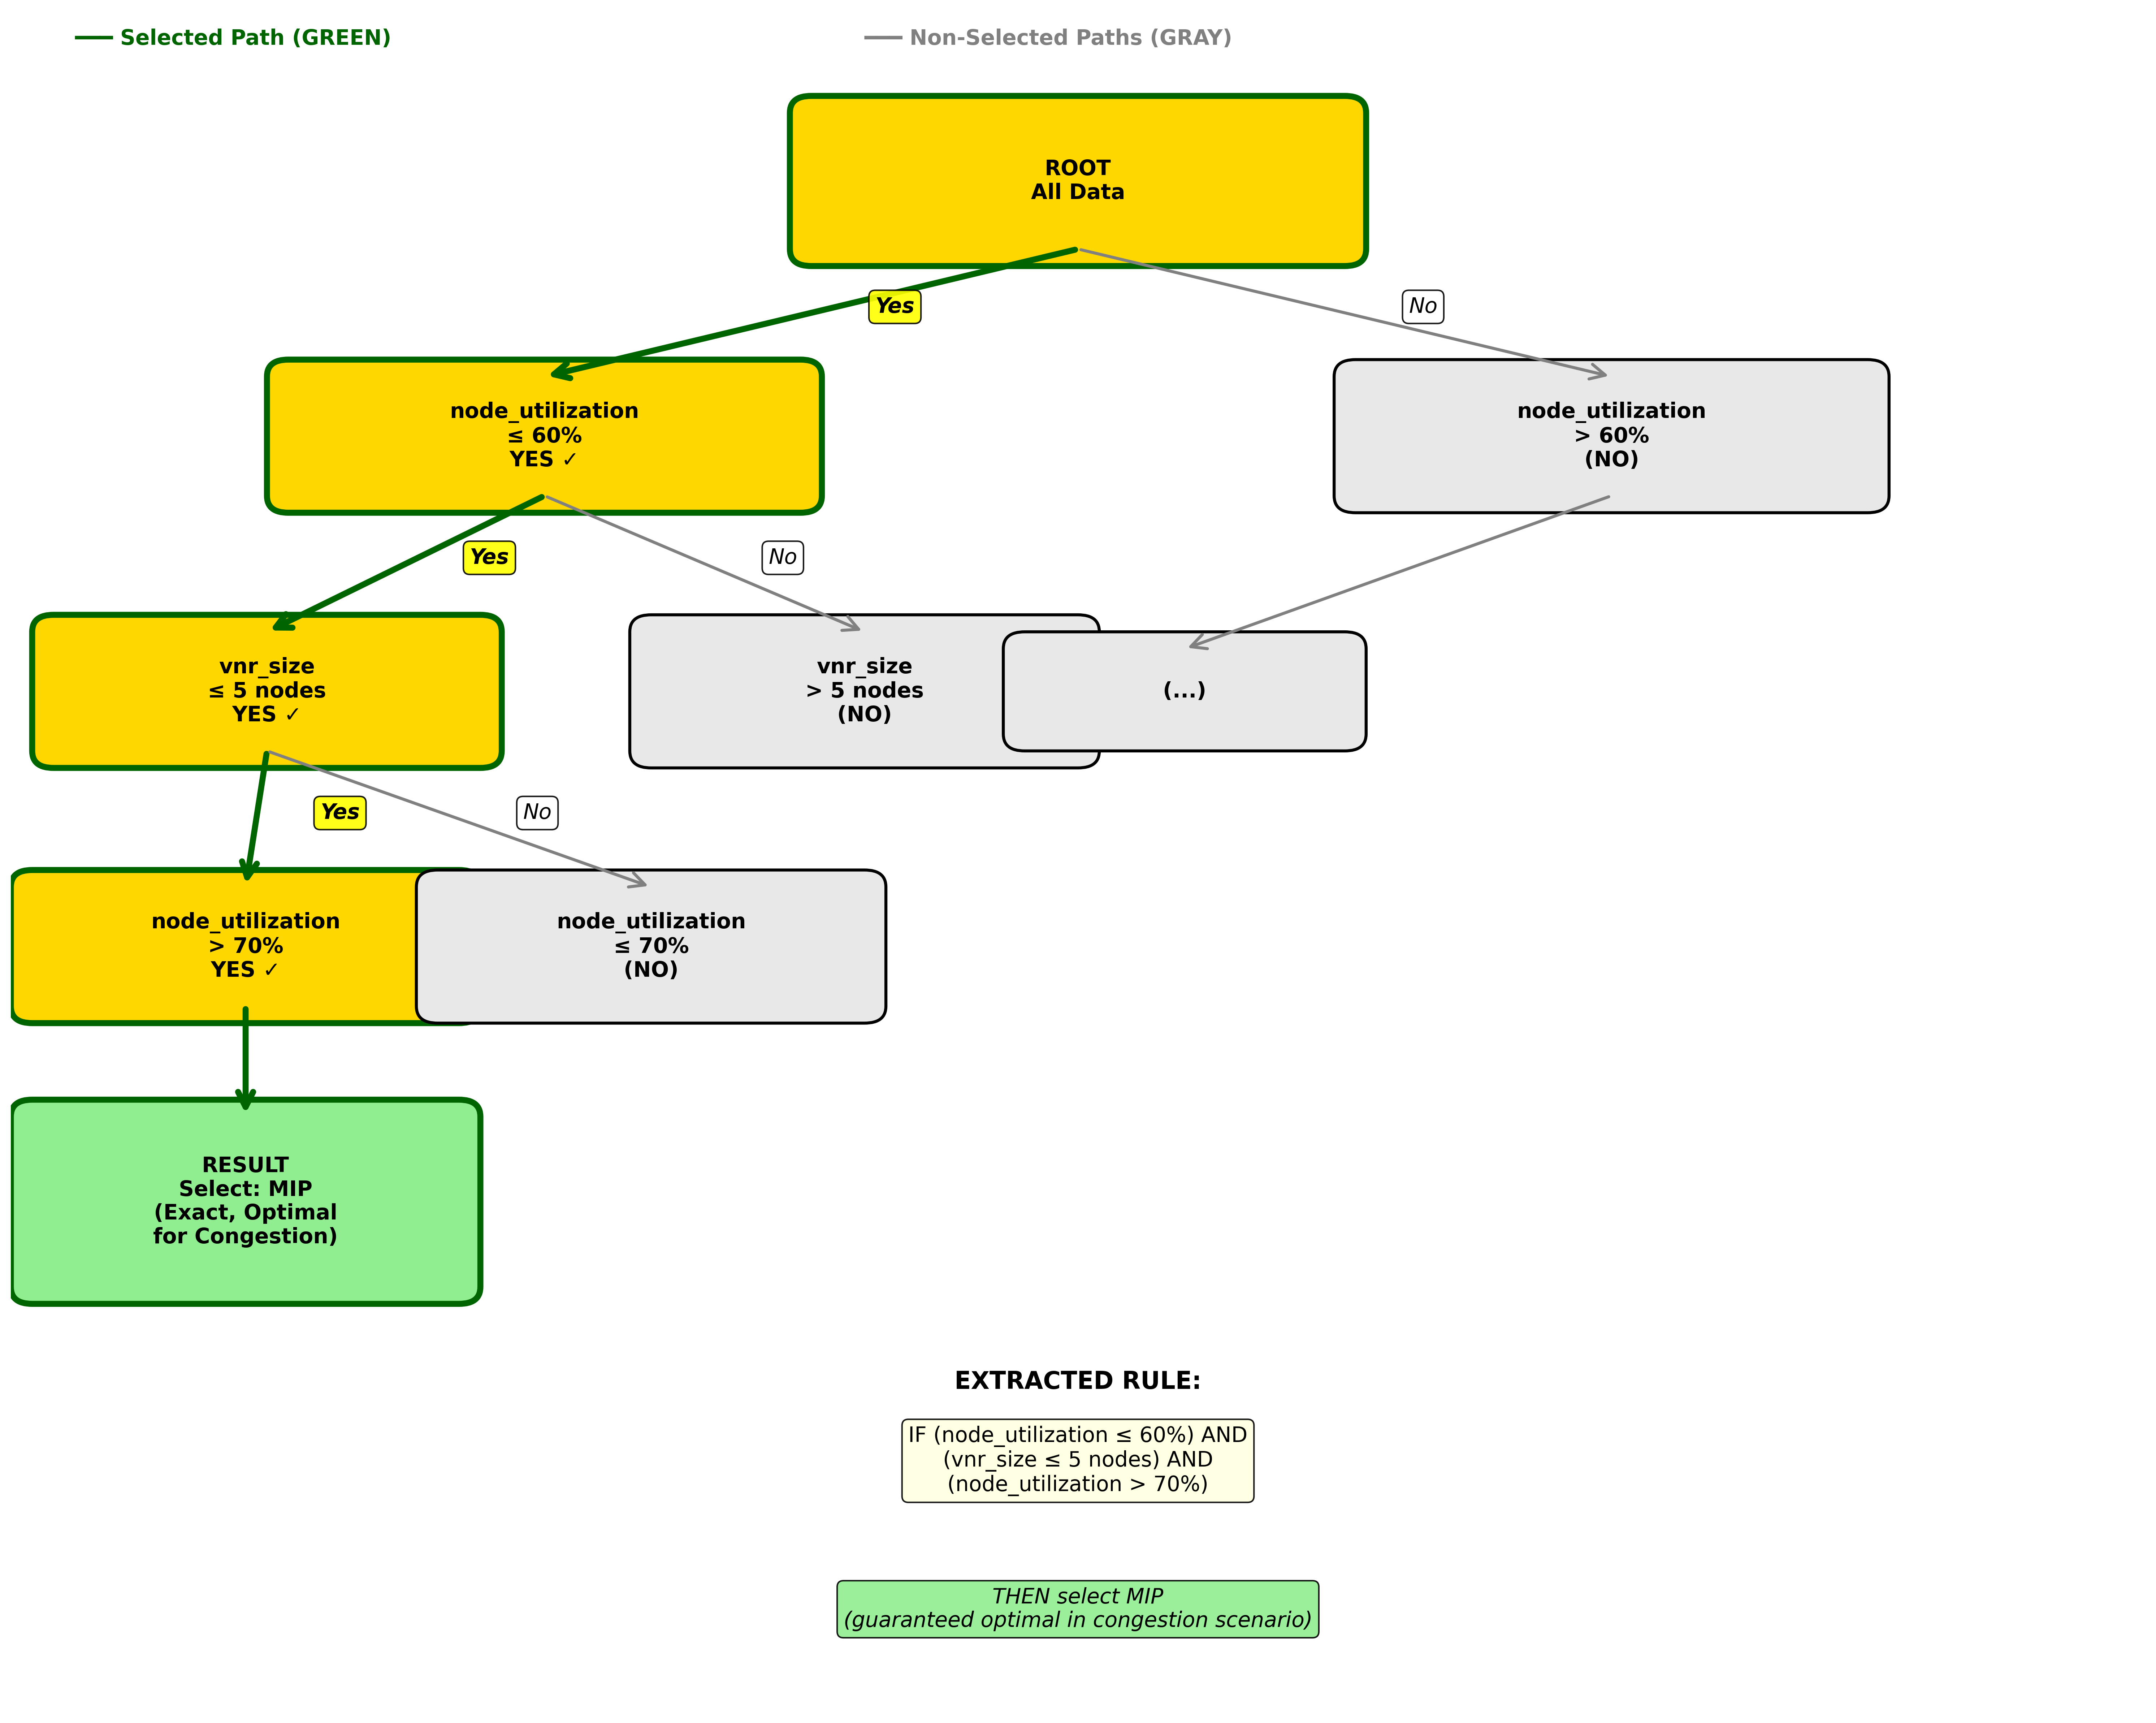
\includegraphics[width=0.665\linewidth]{tree_example_path_en}
    \caption{Example of decision path (root to leaf) in tree for VNE algorithm selection.}
    \label{fig:tree-example-path}
\end{figure*}


\subsubsection{\textcolor{stronggreen}{Why Decision Trees for VNE Selection}}

\textcolor{stronggreen}{Decision trees are chosen in this work not only for their simplicity, but because they directly address the limitations observed in prior automatic algorithm selection approaches. Similar to portfolio-based selectors~\cite{xu2012satzilla} and knowledge-based schedulers for HPC data centers~\cite{koslowski2025knowledge-based}, our method learns from historical executions of existing algorithms, consolidating algorithmic expertise into a data-driven selector. Unlike regression-based scoring functions and deep reinforcement learning policies~\cite{cao2018nfv-deeprl,ijcai-2024-flagvne}, however, each prediction produced by a decision tree corresponds to an explicit rule that can be written as a human-readable conditional statement linking measurable network and request characteristics to a specific algorithm recommendation. This property enables per-topology and per-context analysis of the learned selection policy, which is essential for ZSM-compliant operation~\cite{white2024zerotough} and regulatory audits.}

\textcolor{stronggreen}{In addition to interpretability, decision trees provide low inference latency and modest training requirements. In these experiments, prediction latency remains in the sub-millisecond range, making the approach suitable for online VNE decisions without introducing additional bottlenecks. Trees can also be trained with relatively small datasets and limited hyperparameter tuning when compared to deep learning and ensemble methods. Alternative models such as random forests, gradient-boosted trees, or deep RL may achieve marginally higher predictive accuracy in some scenarios, but they reintroduce black-box behavior and make the extraction of concise decision rules substantially more difficult. Given the emphasis on explainability, auditability, and zero-touch operation in this work, decision trees offer a favorable trade-off between performance, latency, and transparency.}

\subsection{Multi-Objective Optimization}
\label{subsec:multiobj}

The selection of which algorithm to use should not consider only a single performance metric. In real production environments, multiple objectives compete simultaneously: VNR acceptance rate, resolution time, and resource consumption. Approaches that optimize a single objective frequently neglect others, causing system imbalance. The proposed strategy employs multiple specialized trees, each optimized for a specific objective, allowing the system to adapt priorities at runtime according to operational requirements.

\section{Related Work}
\label{sec:RelatedWork}

This section positions the work in relation to existing literature in VNE, algorithm selection, and network automation.
Table~\ref{tab:related-work} synthesizes the comparative analysis between related work and the proposed approach.

\subsection{Algorithm Selection}
\label{subsec:alg-selection}

The algorithm selection problem was formalized by Rice~\cite{rice1976algorithm}, who established the conceptual \textit{framework}: given a problem space, a set of algorithms, a descriptive \textit{feature} space, and performance metrics, determine which algorithm is most appropriate for each problem. This \textit{framework} underlies the approach proposed in this work.
%
Thw work~\cite{xu2012satzilla} develop SATzilla, a portfolio-based selector for satisfiability (SAT) problems, showing that dynamic selection produces significant gains over single algorithms. Similarly, \cite{koslowski2025knowledge-based} apply machine learning techniques for the adaptive selection of scheduling policies in high-performance computing (HPC) infrastructures, showing that the consolidation of multiple strategies offers superior adaptability. This paradigm applies equally to the VNE domain.

\textcolor{stronggreen}{Prior work on automatic algorithm selection and portfolio-based methods~\cite{rice1976algorithm,xu2012satzilla} provides strong evidence that data-driven selectors can improve robustness and average performance across heterogeneous instances. Surveys on automated algorithm selection~\cite{kotthoff2012algorithm,kerschke2019comprehensive} and automatic choice of machine learning algorithms and hyperparameters~\cite{feurer2019automated,vanschoren2018meta} show that selector models and meta-learning frameworks consistently outperform fixed baselines by adapting decisions to instance-level features. In the HPC context, knowledge-based schedulers~\cite{koslowski2025knowledge-based} learn from historical traces using regression and classification to score scheduling policies and define execution orders, improving indicators such as bounded slowdown, waiting time, and turnaround time. These works demonstrate that learning from past decisions is a powerful strategy.}


\subsection{Multi-Objective Optimization in Networks}
\label{subsec:multiobj-networks}

The operational realities of modern networks require simultaneous optimization of multiple objectives: acceptance rate, revenue-cost ratio, average revenue, and processing time. Classical approaches in VNE typically optimize a single objective, neglecting trade-offs with others.

The works~\cite{song2020multiobjective} and~\cite{belgacem2016multiobjective} explore multi-objective optimization for VNE and resource allocation in virtualized networks. However, these approaches frequently use evolutionary algorithms or dynamic integer programming, which suffer from computational complexity during online operation. The proposed approach differentiates itself by employing independent models for each objective, allowing operators to select at runtime which priority to optimize.

\subsection{\textit{Machine Learning} and Reinforcement Learning in Networks}
\label{subsec:ml-networks}

Machine learning has become an important tool for network automation. Initially,~\cite{cao2018nfv-deeprl} apply \textit{Deep Reinforcement Learning} (DRL) for dynamic resource allocation in Network Function Virtualization (NFV).
In turn,~\cite{ijcai-2024-flagvne} propose FlagVNE, a flexible RL framework for VNE with multiple policies.

Although DRL offers adaptability, it faces critical challenges for production: long training time (millions of episodes for convergence), lack of interpretability (decisions function as black box), unstable convergence in dynamic environments, and high inference latency (inadequate for real-time decisions).
Recent work on autonomous network systems recognizes that interpretability is a critical requirement for regulated environments~\cite{white2024zerotough}.

\subsection{Zero-Touch Automation}
\label{subsec:zerotouchj}

The concept of Zero-Touch Network and Service Management (ZSM) was formalized by ETSI since 2017, referring to the operation of network systems with minimal human intervention, through programmable control, virtualization, and closed-loop feedback.
%
Industry research indicates that reducing manual intervention can decrease operational costs by up to 40\%.
However, the gap between research and production remains: RL systems achieve high performance, but lack adequate interpretability for critical operations.

RSCAT~\cite{diel2023rscat} proposes zero-touch automation for congestion control in networks using actor-critic reinforcement learning and software defined networking.
RSCAT shows that combining machine learning and classical techniques can enable autonomous operation, similarly to the approach proposed in this work for contextual selection of VNE algorithms.

\textcolor{stronggreen}{In the context of zero-touch operation, high predictive accuracy alone is not sufficient: automated controllers must also provide transparent and auditable decisions~\cite{white2024zerotough}. Existing learning-based automation solutions, including deep reinforcement learning controllers~\cite{cao2018nfv-deeprl,ijcai-2024-flagvne} and knowledge-based schedulers~\cite{koslowski2025knowledge-based,diel2023rscat}, predominantly expose aggregate performance indicators and policy-selection frequencies, but do not reveal the internal reasoning that leads to each decision. This misalignment between opaque decision processes and the need for accountable, explainable automation in ZSM scenarios motivates the use of models that can both adapt to context and expose their decision logic. Our proposal is designed with this requirement in mind, using multi-objective decision trees that learn from historical data while producing explicit decision paths that operators and regulators can inspect and validate.}

\subsection{Discussion}

Table~\ref{tab:related-work} synthesizes a comparative analysis between related work and the proposed approach according to six critical dimensions for production systems.
This work differentiates itself by combining established concepts---algorithm selection, decision trees, and multi-objective optimization---applied to VNE to create a practical and operational solution. The main distinctive contributions include:
\begin{itemize}
    \item Multi-Objectivity: Three specialized models, not just acceptance optimization. Operators can adapt priorities at runtime as operational conditions change.

    \item Contextual Adaptability: Selection based on real network state (utilization, fragmentation) and request characteristics (size, connectivity), not just VNR characteristics.

    \item Complete Interpretability: Unlike RL/DL approaches (black box), each decision can be explained to operators through explicit paths in the decision tree.

    \item Computational Efficiency: Training in seconds (not millions of episodes), inference in sub-milliseconds ($<$1ms), enabling real-time \textit{online} operation.

    \item Practical Validation: Presents real improvement in acceptance rate (+5.73pp) in a realistic simulated environment with 8,000 virtual network requests in three topologies.
\end{itemize}

\begin{table*}[t]
\centering
\scriptsize
\caption{Comparative Analysis: Related Work vs Proposed Approach (six critical dimensions)}
\label{tab:related-work}
\begin{tabular}{lcccccc}
\toprule
\textbf{Work} & \textbf{ML Type} & \textbf{Adaptive} & \textbf{Multi-Obj.} & \textbf{Interpretable} & \textbf{Latency} & \textbf{Prod. Ready} \\
\midrule
Fischer (VNE Survey) & Comparison & No & No & Yes & - & No \\
Rice (Portfolio) & Algorithm & Yes & No & Yes & - & Conceptual \\
SATzilla & Trees & Yes & No & Yes & Low & Yes \\
Cao et al. (DRL) & Deep RL & Yes & No & No & High (50ms+) & No \\
FlagVNE (DRL) & Deep RL & Yes & No & No & Very High (100ms+) & No \\
\midrule
\textbf{This Work} & \textbf{Multi-Obj. Trees} & \textbf{Yes} & \textbf{Yes (3 obj.)} & \textbf{Yes} & \textbf{$<$1ms} & \textbf{Yes} \\
\bottomrule
\end{tabular}
\end{table*}


\section{Methodology}
\label{sec:Proposal}

The methodology consists of four main steps:

\begin{enumerate}
        \item \textbf{Data Collection}: Execute eight VNE algorithms implemented in the Virne simulator~\cite{wang2024virne}---representing three algorithm classes: exact methods (\textit{MIP}), meta-heuristics (\textit{GA-Meta, PSO-Meta, SA-Meta, MCTS}), and heuristics (\textit{PL-Rank, RW-Rank-BFS, D-Round})---on three distinct physical network topologies: two structured \textit{datacenter} topologies (\textit{Tree, Fat-Tree with k=4}) and one random topology. This diversity of algorithms and topologies ensures the decision tree has sufficient variability to learn contextual patterns and generalize across different network scenarios. Detailed performance data are collected in each scenario for model training, validation, and testing.
    \item Feature Engineering: Extract 27 relevant characteristics from VNRs, network state, and topological context.
    \item Multi-Objective Training: Create three specialized models, Request Acceptance Rate (RAC), Long-term Revenue-to-Cost Ratio (LRC) and Long-term Average Revenue (LAR), each optimizing specific performance criteria.
    \item Online Prediction: For each new VNR, use the extracted context to dynamically select the most appropriate VNE algorithm through the model that optimizes the desired criterion.
\end{enumerate}

\subsection{Simulation Data Generation}

Data were collected using the Virne~\cite{wang2024virne} platform, a comprehensive benchmarking framework for Network Function Virtualization Resource Allocation (NFV-RA) problems. Virne offers highly customizable simulations for various network scenarios, including cloud datacenters, edge computing, and 5G networks. The platform implements more than 30 NFV-RA algorithms in a modular and extensible architecture, providing an \textit{event-driven} simulation environment that models the physical network (PN) infrastructure and sequential virtual network requests (VNRs). Each VNR arrival is treated as a discrete event, creating an instance that the NFV-RA algorithm must solve, evaluating solution feasibility and updating network resources.

Simulations were executed with eight VNE algorithms on three distinct topologies, commonly used in \textit{datacenters}:

\begin{itemize}
    \item Tree: A binary tree with 32 hosts and 31 switches (63 nodes)
    \item Fat-Tree: \textit{Datacenter} with k=4 (16 servers, 20 switches, 36 nodes)
    \item Waxman-16: Random network with 16 nodes and 500 links
\end{itemize}

Simulations were configured with homogeneous resources (CPU and memory) uniformly distributed on physical nodes. VNRs were generated with variable size (uniform distribution between 2 and 10 virtual nodes), 50\% connectivity between virtual nodes, and resource demands following realistic distributions. The system simulates sequential VNR arrivals with arrival rate according to Poisson distribution, where each request has a stochastic lifetime. Virne automatically evaluates the feasibility of each solution proposed by the algorithms, verifying node and link capacity constraints, and calculates standardized performance metrics (RAC, LRC, LAR, AST) for each execution.

For each combination of algorithm and topology, ten repetitions were executed with different random seeds, totaling approximately 8,000 unique VNRs after deduplication. This approach ensures statistical robustness and captures the variability inherent to stochastic algorithms and dynamic characteristics of virtual network requests.

\subsection{Feature Engineering}

A set of 27 features was carefully selected, divided into categories:

\begin{itemize}
    \item VNR Characteristics (9 features): number of nodes, number of links, size ratio, average demand per node, average demand per link, connectivity, total demand, node/link ratio, expected lifetime.

    \item Physical Network State (4 features): available resources, node utilization, link utilization, overall utilization.

    \item System State (3 features): number of active VNRs, system load, active physical nodes.

    \item Heterogeneity and Fragmentation (10 engineered features): Gini indices for resource distribution, memory fragmentation, topological diversity indices.

    \item Context (1 feature): topology type.

\end{itemize}

\subsection{Multi-Objective Architecture}

Instead of a single classification model, we employ three specialized models, each optimized for a specific objective:

\begin{itemize}
    \item RAC: Maximize virtual network request acceptance rate
    \item LRC: Maximize long-term revenue-cost ratio
    \item LAR: Maximize long-term average revenue
\end{itemize}

Each model is a decision tree trained independently on historical simulation data. During online operation, the operator (or automatic policy) selects which objective to prioritize, and the corresponding model predicts the best algorithm.

\subsection{Model Training}

The training process was performed independently for each objective (RAC, LRC, LAR), allowing each model to specialize in optimizing its specific metric. Data division was stratified by algorithm class to ensure balanced distribution between training (70\%), validation (15\%), and test (15\%) sets. This stratification is crucial to maintain representativeness of all classes in each partition, especially considering the severe imbalance observed in the data.

Models use \texttt{DecisionTreeClassifier} from scikit-learn with the following optimized hyperparameters:

\begin{itemize}
    \item Maximum depth: 10 (balancing expressiveness and interpretability)
    \item Minimum samples per leaf: 3 (reduced to allow capture of minority classes)
    \item Minimum samples for split: 6 (allows splits with fewer samples)
     \item Gini impurity for \textit{feature} selection, measuring class separation with values from 0 for pure nodes to 0.5 for maximum impurity, minimizing impurity to maximize class homogeneity at each split
\end{itemize}

As shown in Table~\ref{tab:algorithm-summary}, no algorithm is universally optimal, evidencing the need for contextual selection. This observation justifies the dynamic algorithm selection approach proposed in this work.

\begin{table}[H]
\centering
\tiny
\caption{VNE Algorithm Performance Summary}
\label{tab:algorithm-summary}
\begin{tabular}{lcccc}
\toprule
\textbf{Algorithm} & \textbf{Acc. Rate} & \textbf{Revenue} & \textbf{R2C} & \textbf{Time (s)} \\
\midrule
MIP & 36.8\% & 186.8 & 115.6 & 1.026 \\
PL\_RANK & 29.5\% & 388.4 & 127.4 & 0.661 \\
GA\_META & 27.9\% & 400.6 & 139.8 & 0.603 \\
RW\_RANK\_BFS & 25.8\% & 373.9 & 120.4 & 0.558 \\
SA\_META & 24.6\% & 372.6 & 133.5 & 0.534 \\
MCTS & 23.9\% & 379.7 & 167.0 & 0.468 \\
D\_ROUND & 20.4\% & 365.4 & 246.0 & 0.357 \\
PSO\_META & 20.1\% & 352.1 & 120.0 & 0.309 \\
\bottomrule
\end{tabular}
\end{table}


\subsection{Multi-Metric Comparison of VNE Algorithms}

Different operational contexts (high load, limited resources, latency requirements) require different trade-offs. Figure~\ref{fig:algorithm-comparison} presents a comprehensive analysis of four complementary metrics for the eight evaluated algorithms:

\begin{figure*}[h]
    \centering
    \includegraphics[width=1.0\textwidth]{algorithm_comparison_all_metrics}
    \caption{Multi-Metric Comparison: Acceptance Rate, Total Revenue, Revenue-Cost Ratio, and Average Time per VNR. The graphs show distribution of results in five simulated executions per algorithm across topologies (Tree, Fat-Tree, Waxman-16). No single algorithm is optimal in all dimensions.}
    \label{fig:algorithm-comparison}
\end{figure*}


\subsubsection{Class Balancing Techniques}

To reduce dataset imbalance, a class balancing techniques was applied.
%
Instead of scikit-learn's default balancing, weights calculated as $w_i = 1/\sqrt{f_i}$ were used, where $f_i$ is the relative frequency of class $i$. This strategy assigns significantly larger weights to rare classes:

\begin{itemize}
    \item Rare classes (\texttt{pso\_meta}, 17 samples): weight 10.0$\times$
    \item Intermediate classes (\texttt{rw\_rank\_bfs}, 39 samples): weight 6.6$\times$
    \item Majority classes (\texttt{ga\_meta}, 987 samples): weight 1.3$\times$
\end{itemize}

For evaluation, weighted F1-Score and F1-Macro (arithmetic mean of F1 of all classes, treating them equally) metrics were used to evaluate balanced performance between classes.

\section{Experimental Results}
\label{sec:Results}

\subsection{Classification Performance}

Table~\ref{tab:classification-metrics} presents the classification metrics obtained for the three considered objectives (RAC, LRC, and LAR):

\begin{table}[H]
\centering
\resizebox{\columnwidth}{!}{%
\begin{tabular}{lcccc}
\toprule
\textbf{Objective} & \textbf{Accuracy} & \textbf{F1-Score} & \textbf{Top-2} & \textbf{Top-3} \\
\midrule
RAC (Acceptance Rate) & 67.26\% & 0.68 & 82.66\% & 85.90\% \\
LRC (Revenue-Cost Ratio) & 54.46\% & 0.55 & 74.55\% & 83.95\% \\
LAR (Average Revenue) & 48.14\% & 0.48 & 67.59\% & 79.09\% \\
\bottomrule
\end{tabular}%
}
\caption{Classification Metrics by Objective (Balanced Models)}
\label{tab:classification-metrics}
\end{table}

Results presented in Table~\ref{tab:classification-metrics} indicate that the RAC objective presents better performance in all metrics, with accuracy of 67.26\% and top-3 accuracy of 85.90\%. The LRC objective presents intermediate performance, while LAR presents lower accuracy (48.14\%), but still with top-3 accuracy of 79.09\%, indicating that the model frequently identifies the best algorithm among the top three options. The performance difference between objectives reflects the distinct complexity of each metric and the inherent variability of algorithms in different contexts.

\subsection{Comparison with \textit{Baseline}}

Classification accuracy was measured for each objective, comparing decision tree performance with the fixed algorithm \textit{baseline}. Figure~\ref{fig:baseline-comparison} presents the results. It is possible to observe that accuracy depends significantly on the chosen fixed algorithm, evidencing the need for contextual selection.

\begin{figure}[H]
\centering
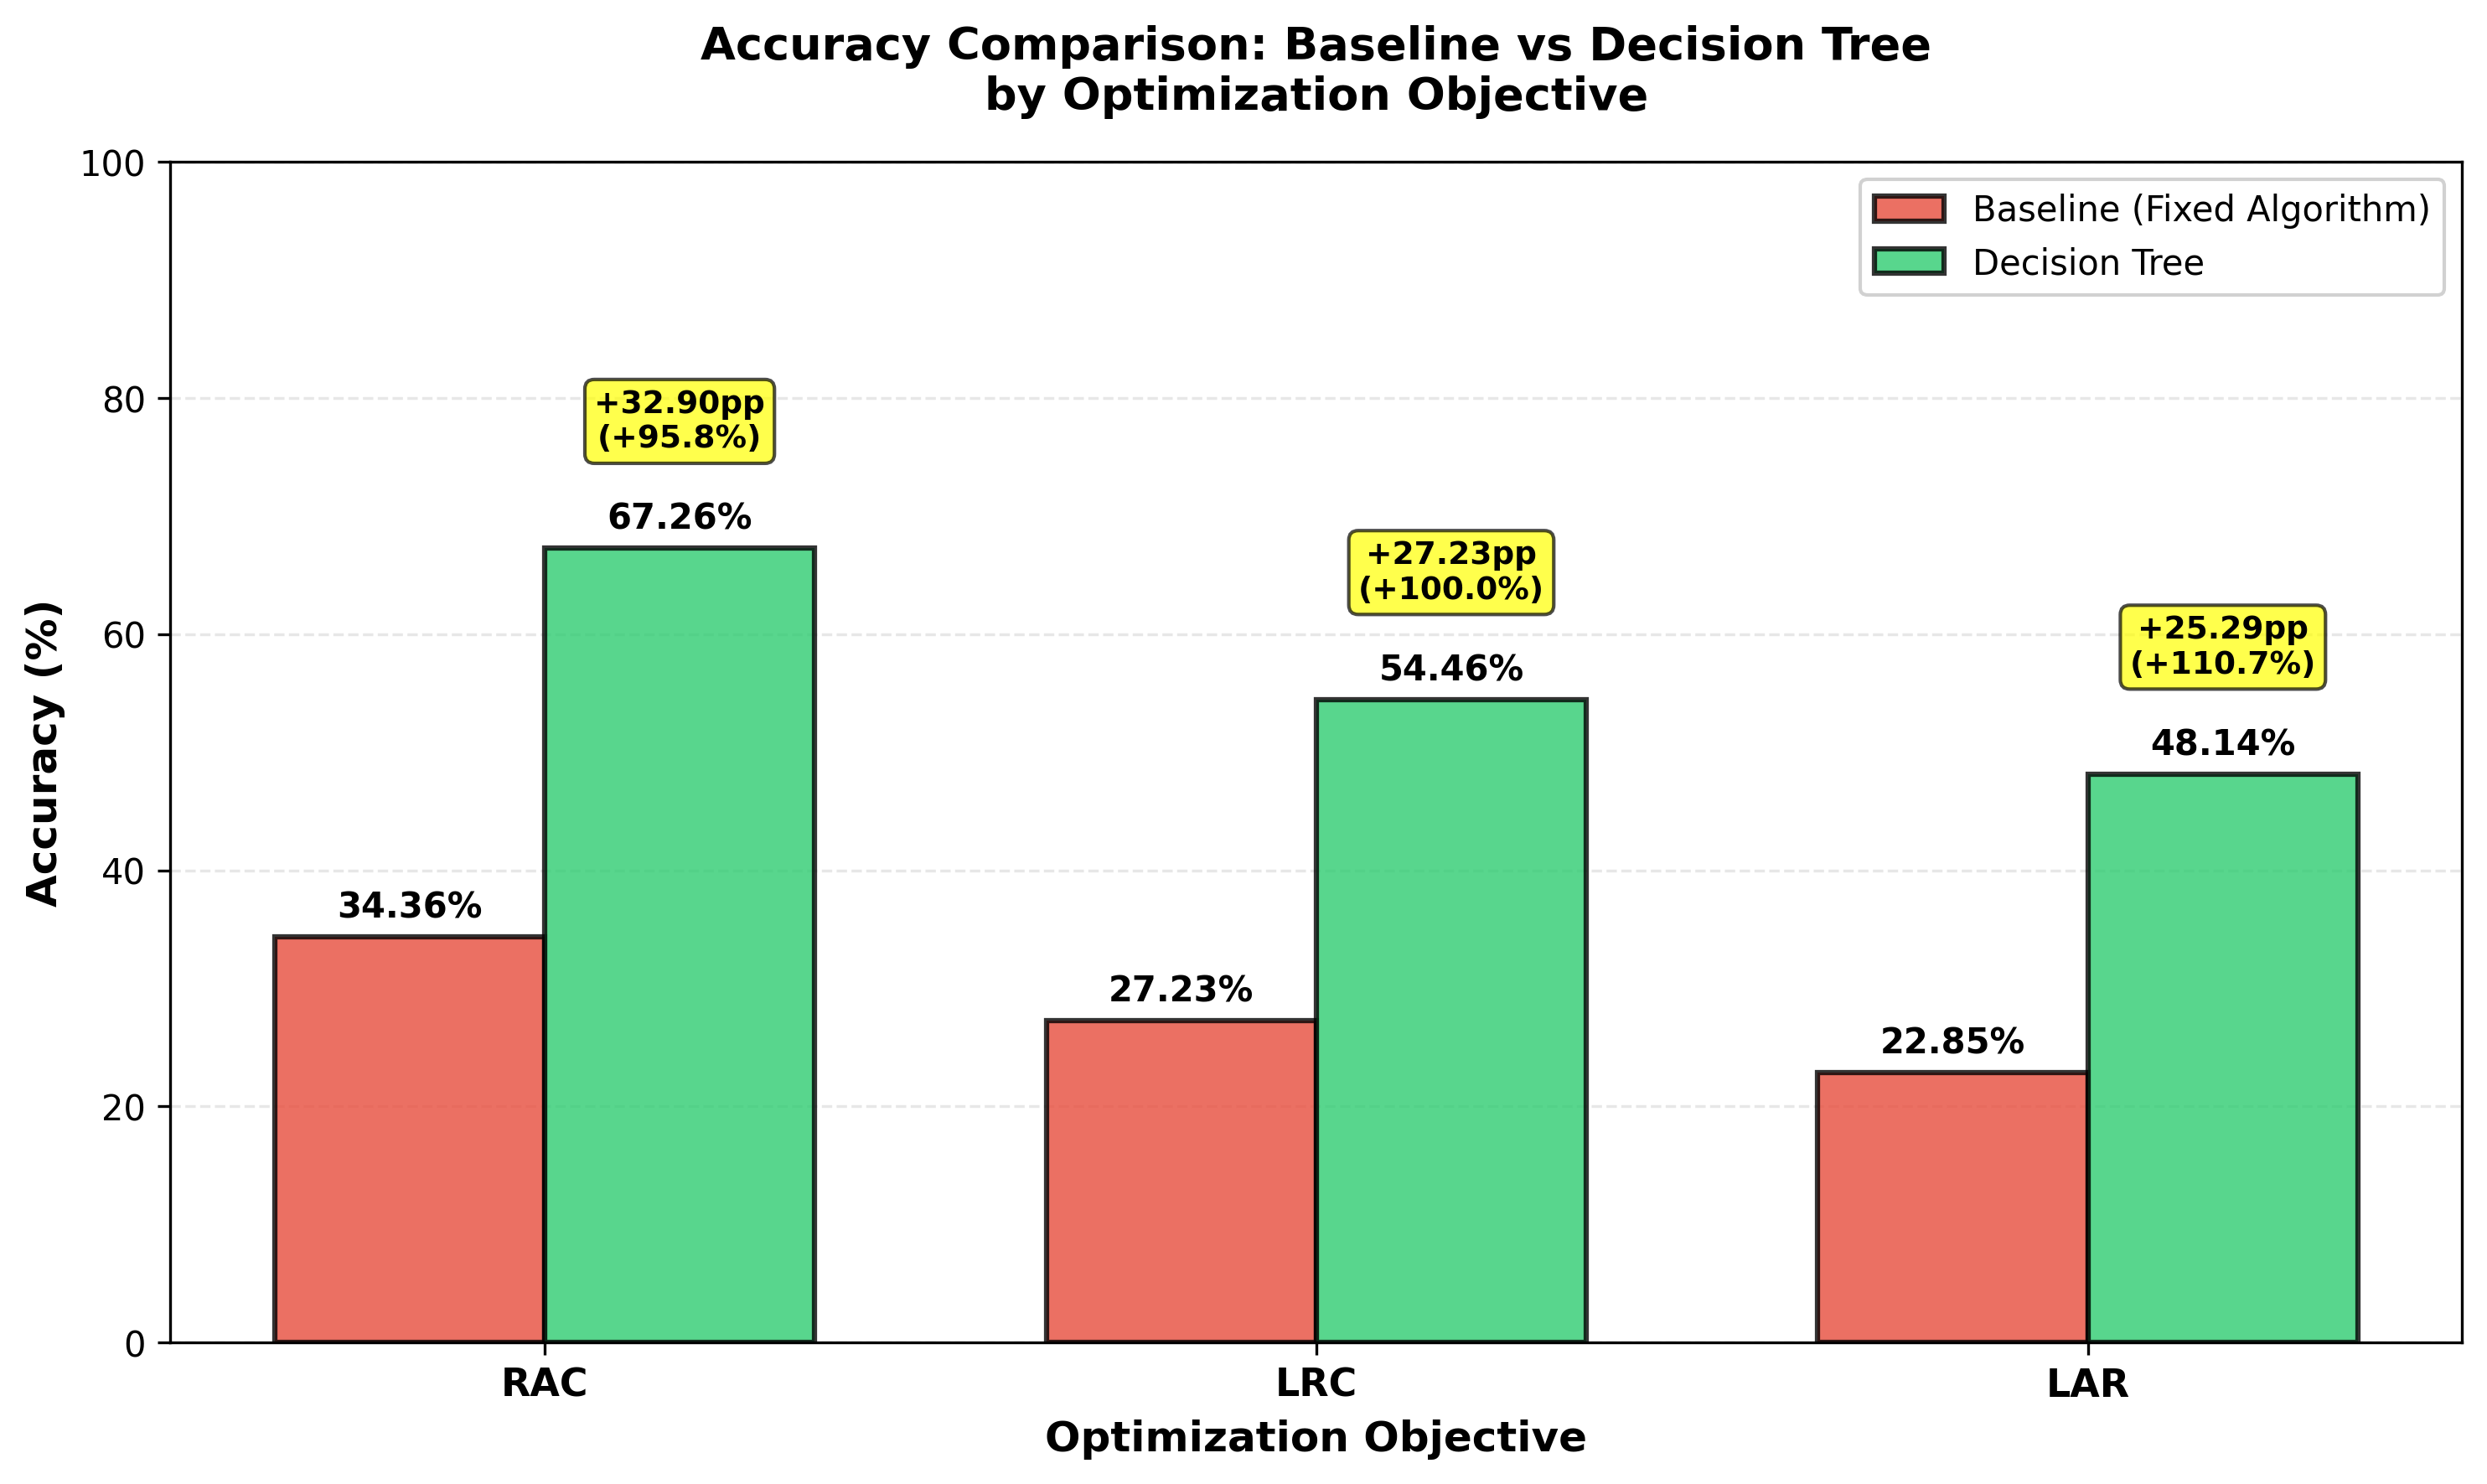
\includegraphics[width=0.95\columnwidth]{baseline_comparison_chart}
\caption{Accuracy Comparison: Baseline vs Decision Tree by Optimization Objective}
\label{fig:baseline-comparison}
\end{figure}

Figure~\ref{fig:baseline-comparison} reveals that contextual selection via decision trees significantly outperforms the use of fixed algorithms. For the RAC objective, the improvement is +32.90 percentage points (+95.8\% relative), while for LRC and LAR the improvements are even more expressive in relative terms (+100.0\% and +110.7\%, respectively). These results confirm that adaptive algorithm selection based on contextual characteristics is fundamental to optimizing system performance.

To validate that gains in classification accuracy translate into real operational performance improvement, performance was evaluated when decision trees are used for algorithm selection in simulated executions.
Figure~\ref{fig:real-performance-improvement} presents the comparison of real performance (using individual values per VNR) between tree-based selection and fixed algorithm baseline.

\begin{figure}[H]
\centering
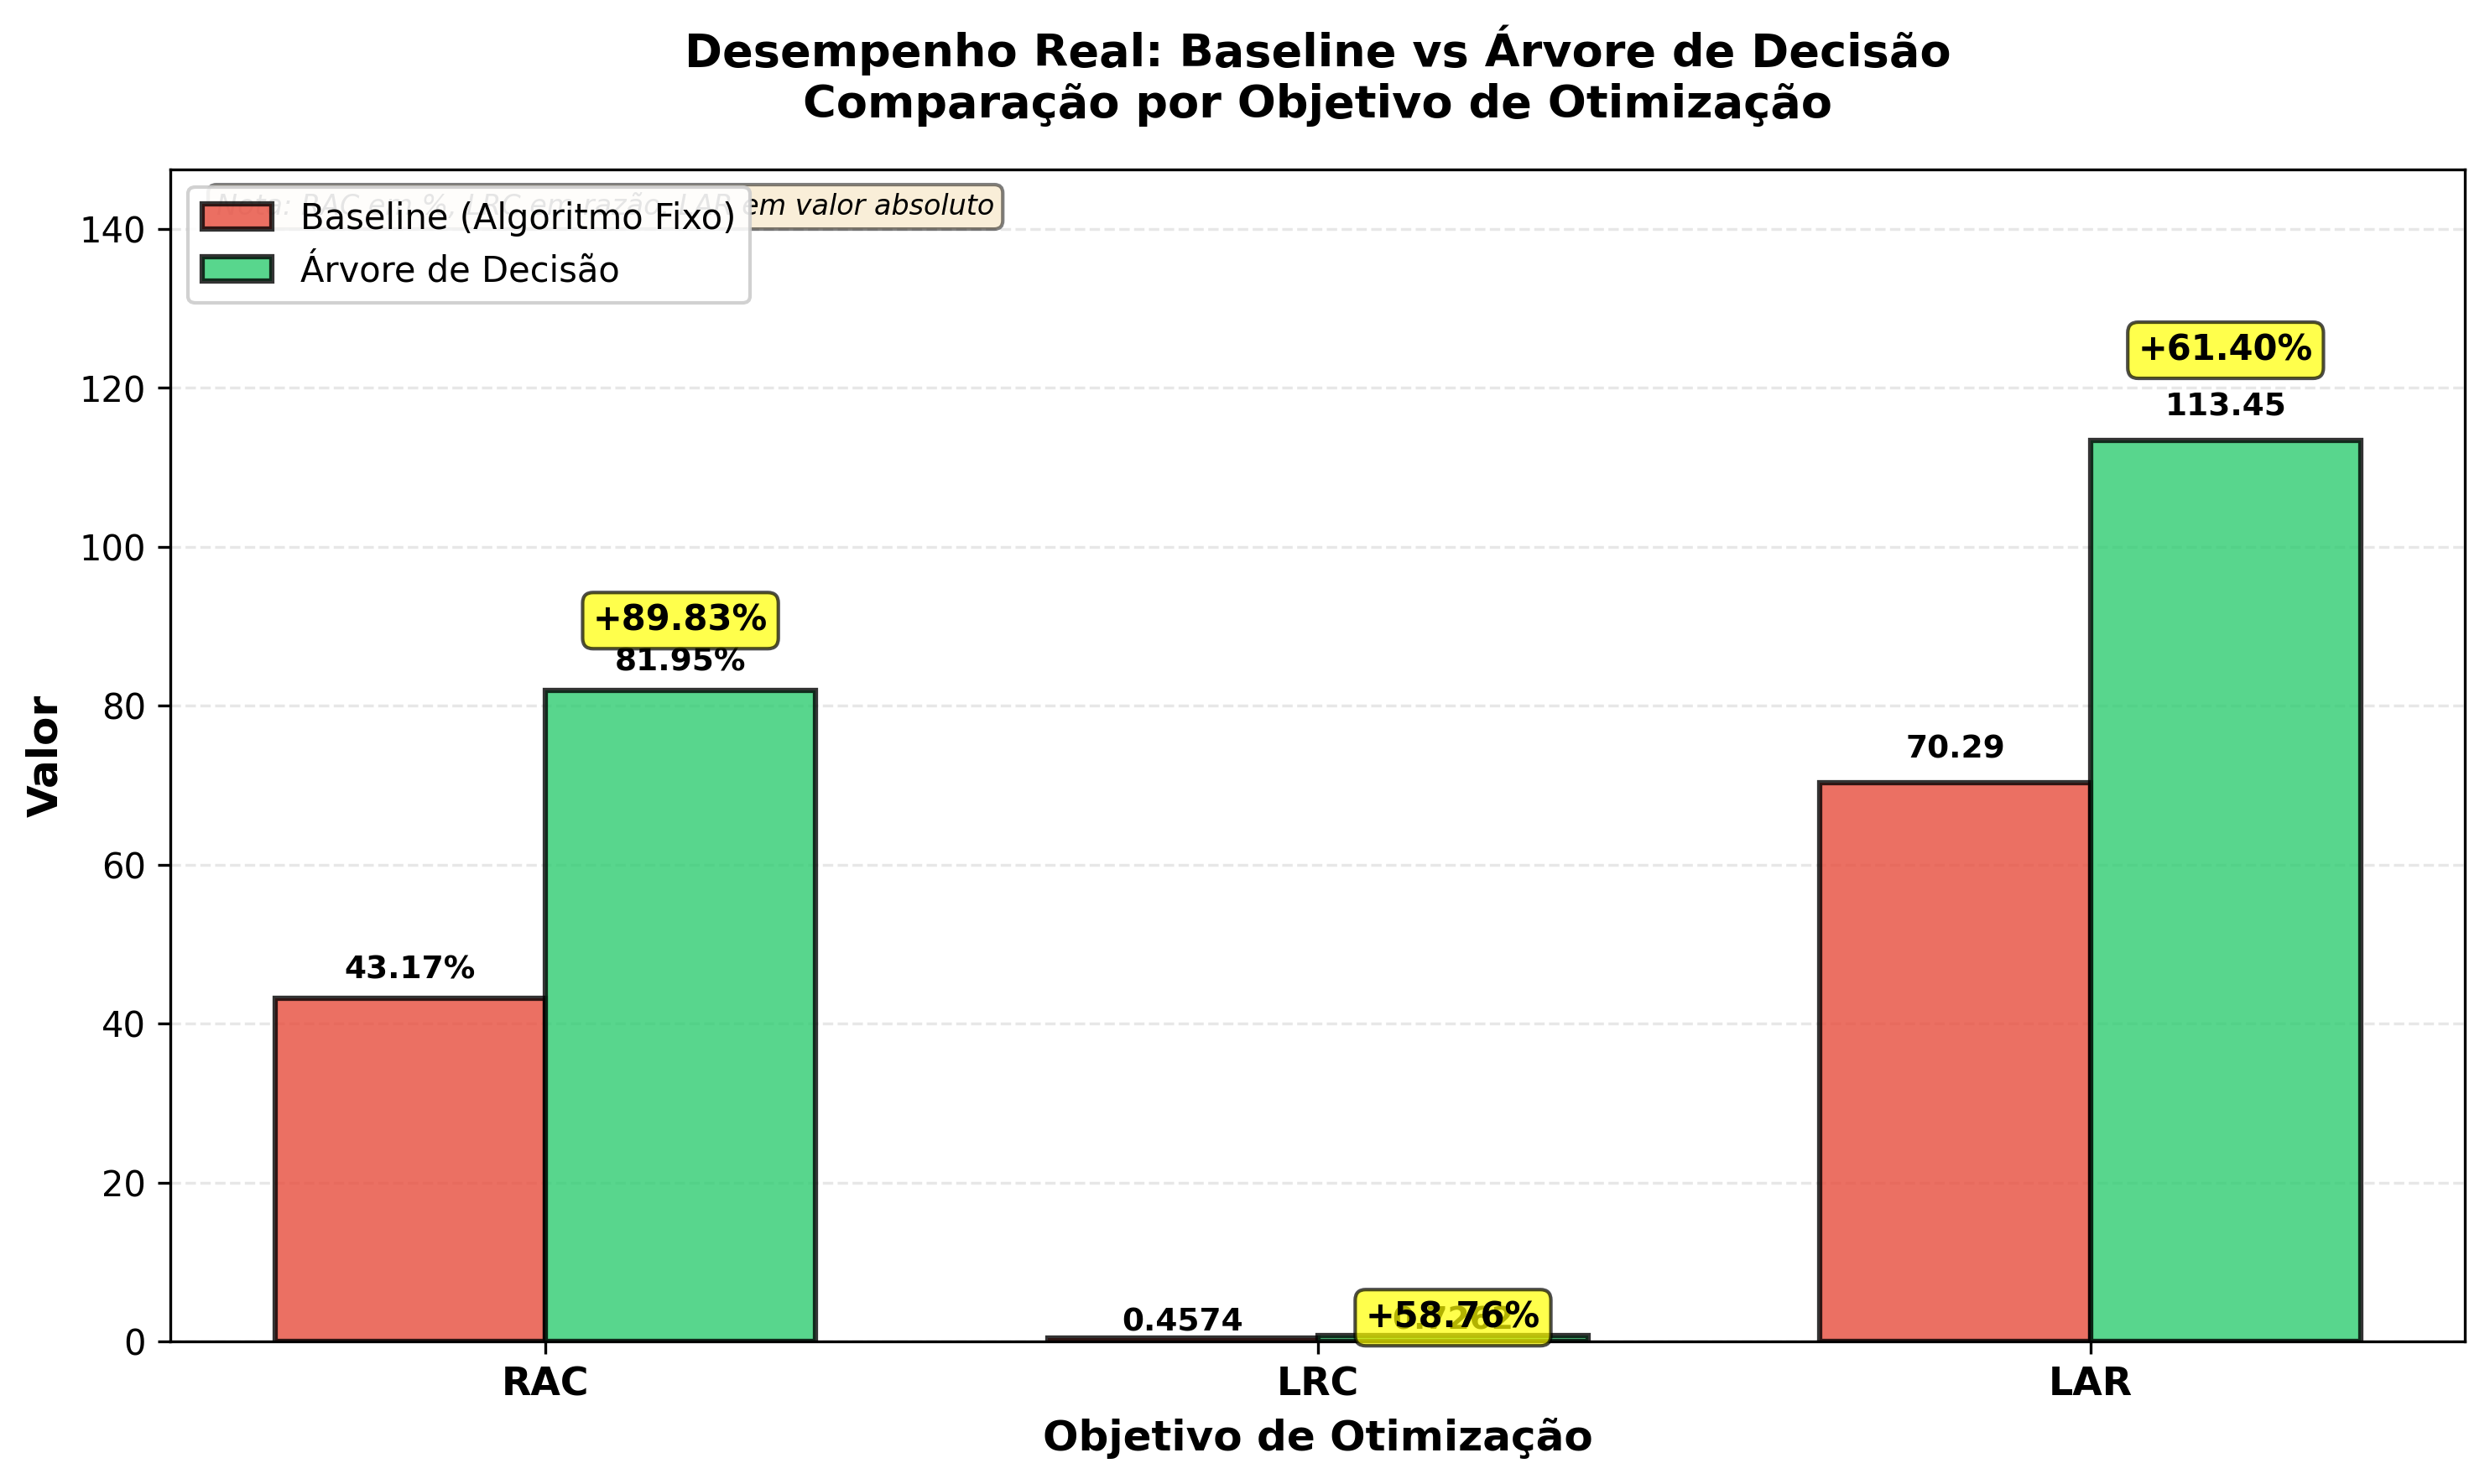
\includegraphics[width=0.95\columnwidth]{real_performance_chart}
\caption{Real Performance: Tree vs Baseline by Optimization Objective}
\label{fig:real-performance-improvement}
\end{figure}

Results show that contextual selection via decision trees produces substantial improvements in real operational performance in all objectives:

\begin{itemize}
    \item RAC: Acceptance rate increases from 43.17\% (fixed algorithm) to 81.95\% (contextual selection), representing an improvement of +89.83\%.
    \item LRC: Revenue-cost ratio increases from 0.4574 to 0.7262, with an improvement of +58.76\%.
    \item LAR: Average revenue increases from 70.29 to 113.45 per VNR, with an improvement of +61.40\%.
\end{itemize}

Results show that contextual selection via decision trees is significantly superior to using a fixed algorithm, with substantial improvements in all evaluated objectives. The approach captures important patterns of algorithm selection based on contextual characteristics of VNRs, allowing dynamic adaptation to different network conditions and resource requirements.

\begin{table}[H]
\centering
\caption{F1-Score per Class - RAC Objective (Balanced Models)}
\label{tab:f1-per-class}
\begin{tabular}{lccc}
\toprule
\textbf{Algorithm} & \textbf{Precision} & \textbf{Recall} & \textbf{F1-Score} \\
\midrule
GA\_Meta & 0.73 & 0.74 & 0.73 \\
MCTS & 0.78 & 0.72 & 0.75 \\
PL\_Rank & 0.77 & 0.66 & 0.71 \\
D\_Round & 0.61 & 0.59 & 0.60 \\
MIP & 0.49 & 0.57 & 0.53 \\
SA\_Meta & 0.43 & 0.56 & 0.49 \\
RW\_Rank\_BFS & 0.67 & 0.25 & 0.36 \\
PSO\_Meta & 0.22 & 0.67 & 0.33 \\
\midrule
F1-Macro & \multicolumn{3}{c}{0.56} \\
F1-Weighted & \multicolumn{3}{c}{0.68} \\
\bottomrule
\end{tabular}
\end{table}

The detailed analysis presented in Table~\ref{tab:f1-per-class} reveals that balancing techniques allow capturing patterns even from minority classes. Algorithms such as GA\_Meta, MCTS, and PL\_Rank present F1-Score above 0.70, indicating good prediction capability. Minority classes such as PSO\_Meta and RW\_Rank\_BFS present lower F1-Score (0.33 and 0.36, respectively), but still above zero, demonstrating that the model can identify patterns even for these classes. F1-Macro of 0.56 and F1-Weighted of 0.68 indicate that the model presents balanced performance across all classes, with greater weight on more frequent classes.

\subsection{Interpretability Analysis}

One of the main advantages of the approach is that each decision can be traced through the decision tree.

Unlike deep neural networks (black box), operators can understand \textbf{exactly why} an algorithm was selected:

\textit{``If VNR size $<$ 30\% of physical network AND node utilization $>$ 70\%, then select MIP (exact, accepts in congestion). Otherwise, if connectivity $>$ 0.5, select GA-Meta.''}

Additionally, \textit{feature} importance analysis reveals which characteristics are most relevant for each objective. For RAC (Request Acceptance Rate) and LRC (Long-Term Revenue-to-Cost), resource efficiency ($resource\_efficiency$) is the most critical \textit{feature}, with importance of 0.13 and 0.11 respectively. In the case of LAR (Long-Term Average Revenue), VNR link demand ($v\_net\_demand\_per\_link$) and total demand ($v\_net\_total\_demand$) are the dominant \textit{features}. These findings confirm that different objectives prioritize distinct characteristics of VNRs and physical network state. Figure~\ref{fig:feature-importance-rac} exemplifies \textit{feature} importance for the RAC objective, while Figures~\ref{fig:feature-importance-lrc} and~\ref{fig:feature-importance-lar} present results for the remaining objectives.

\setlength{\floatsep}{5pt}
\setlength{\intextsep}{5pt}
\setlength{\textfloatsep}{5pt}
\begin{figure}[!htb]
    \centering
    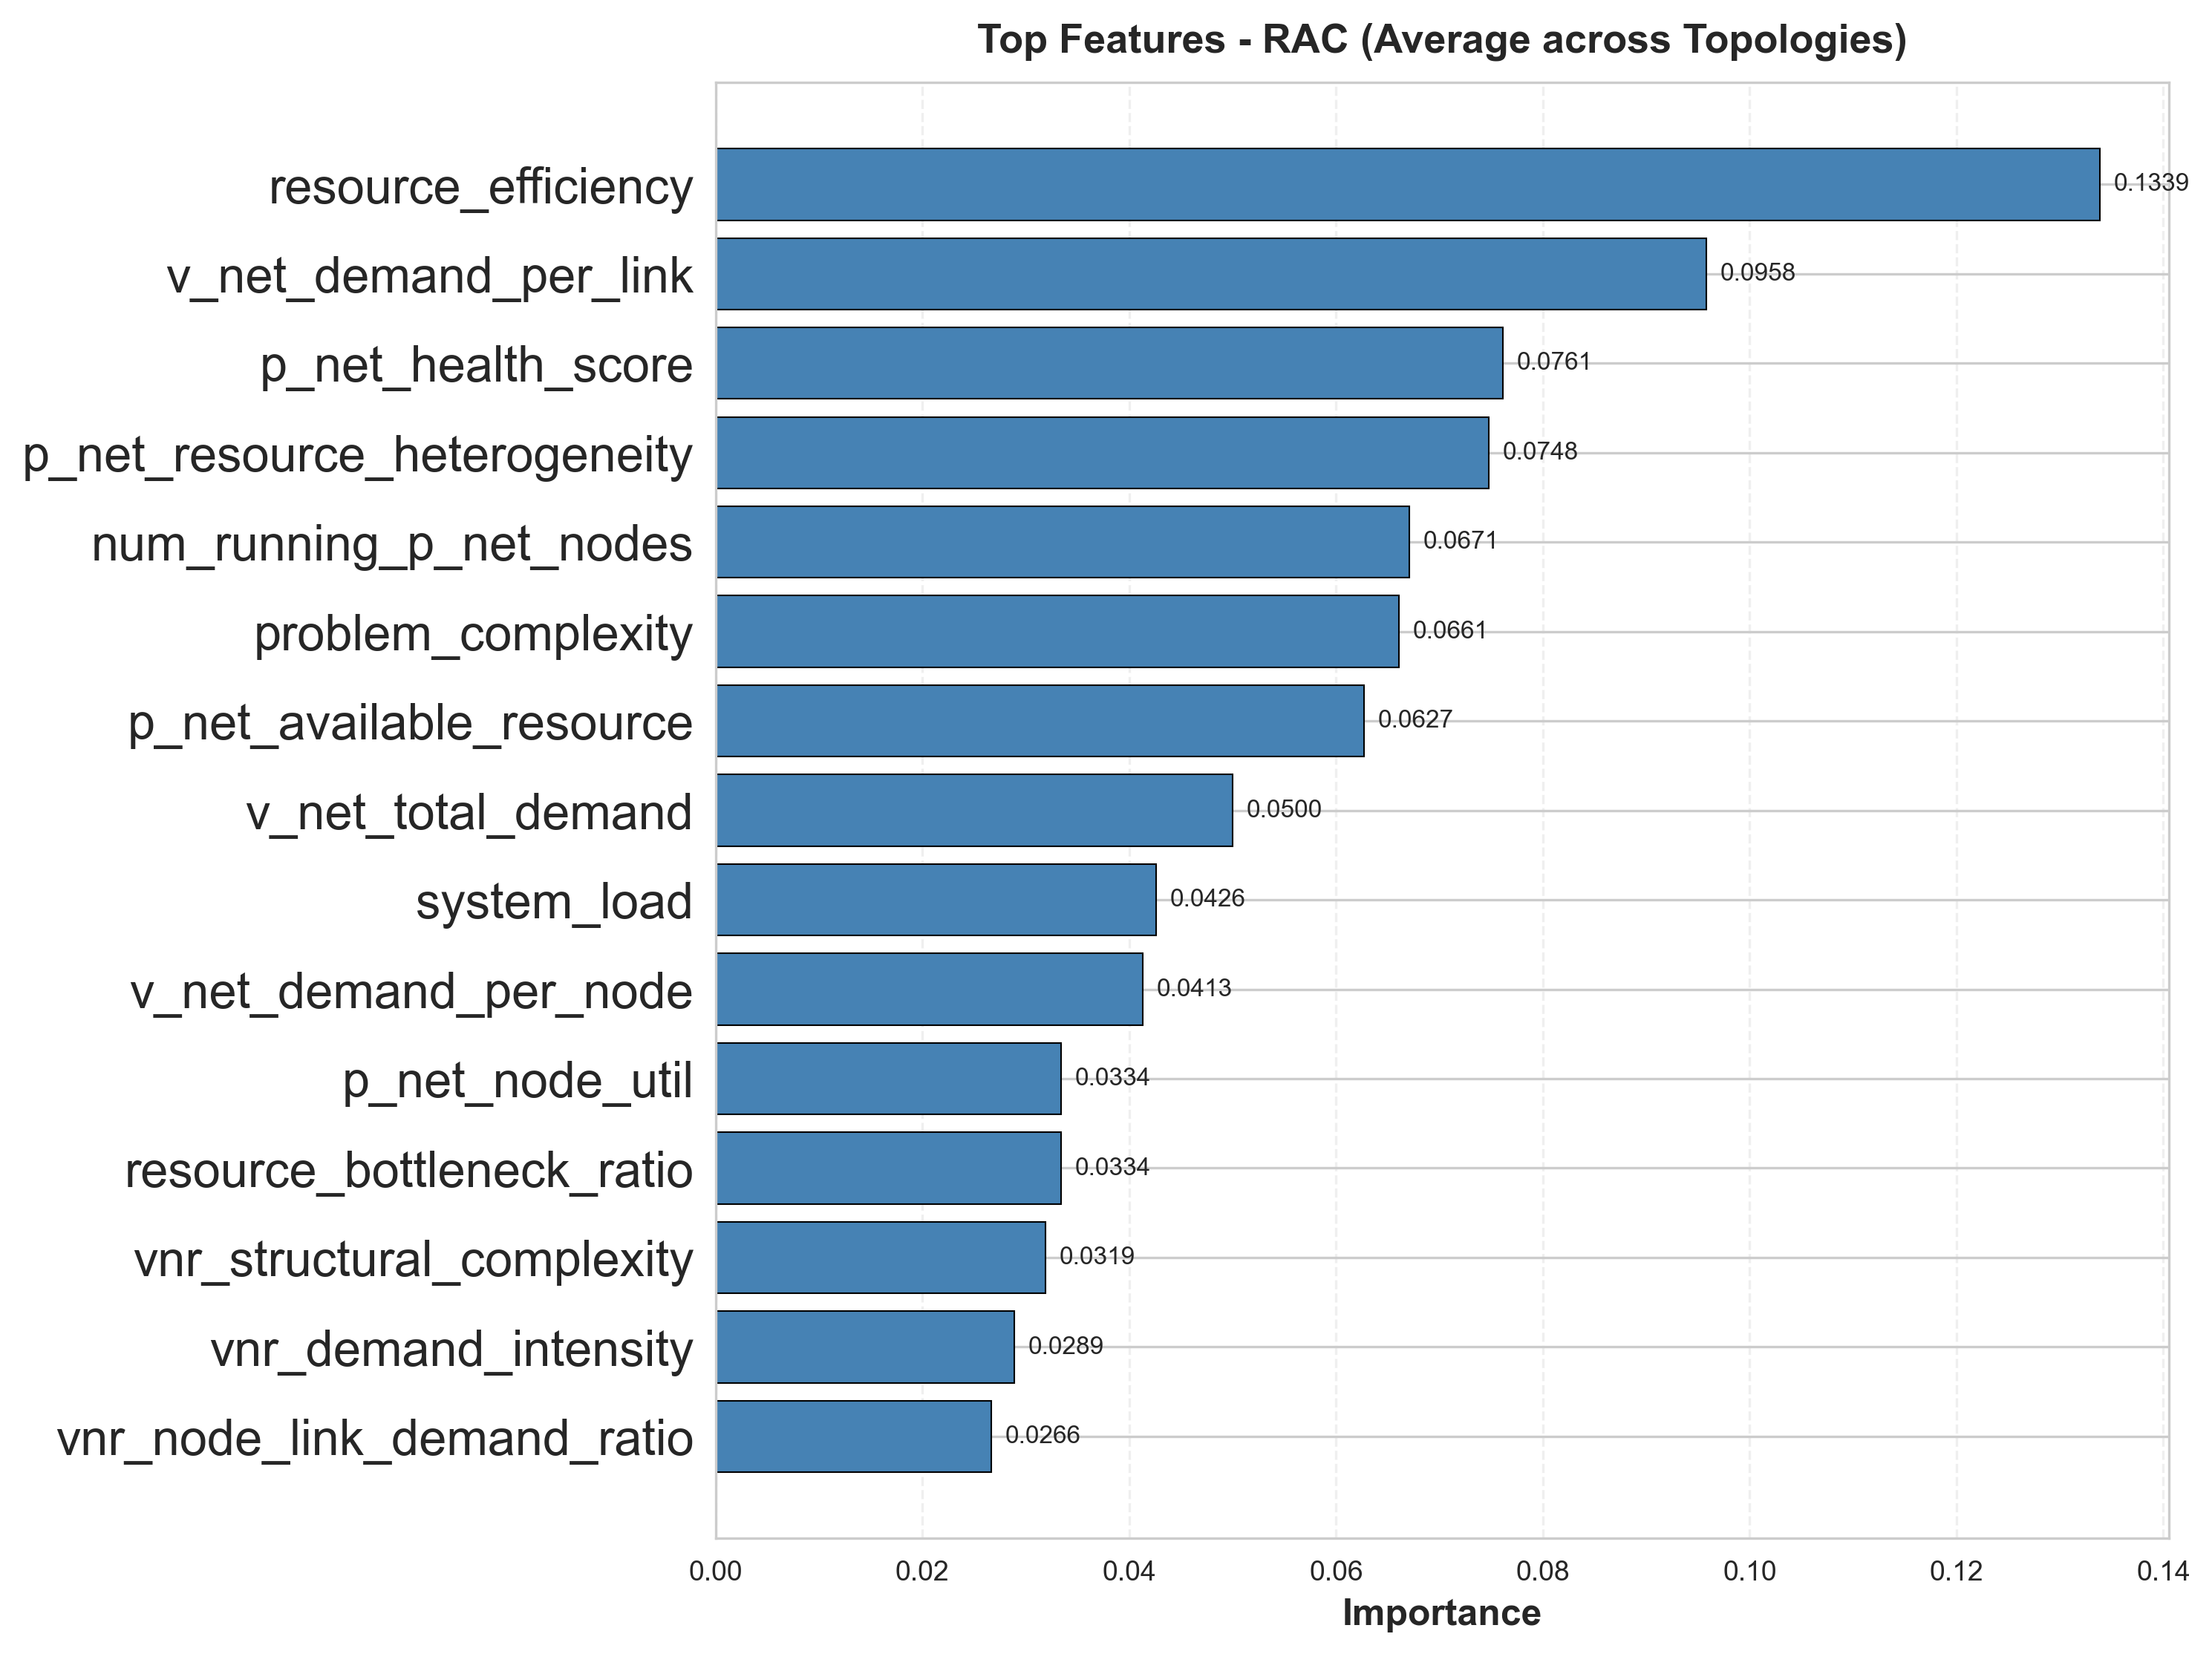
\includegraphics[width=0.95\columnwidth]{per_objective_rac}
    \caption{Feature Importance - RAC (Request Acceptance Rate). The top 15 most important features (average across topologies) for the RAC objective. Resource efficiency ($resource\_efficiency$) is the most critical feature with importance of 0.134, followed by VNR link demand ($v\_net\_demand\_per\_link$) with 0.096.}
    \label{fig:feature-importance-rac}
\end{figure}
\vspace{-2cm}

\begin{figure}[H]
    \centering
    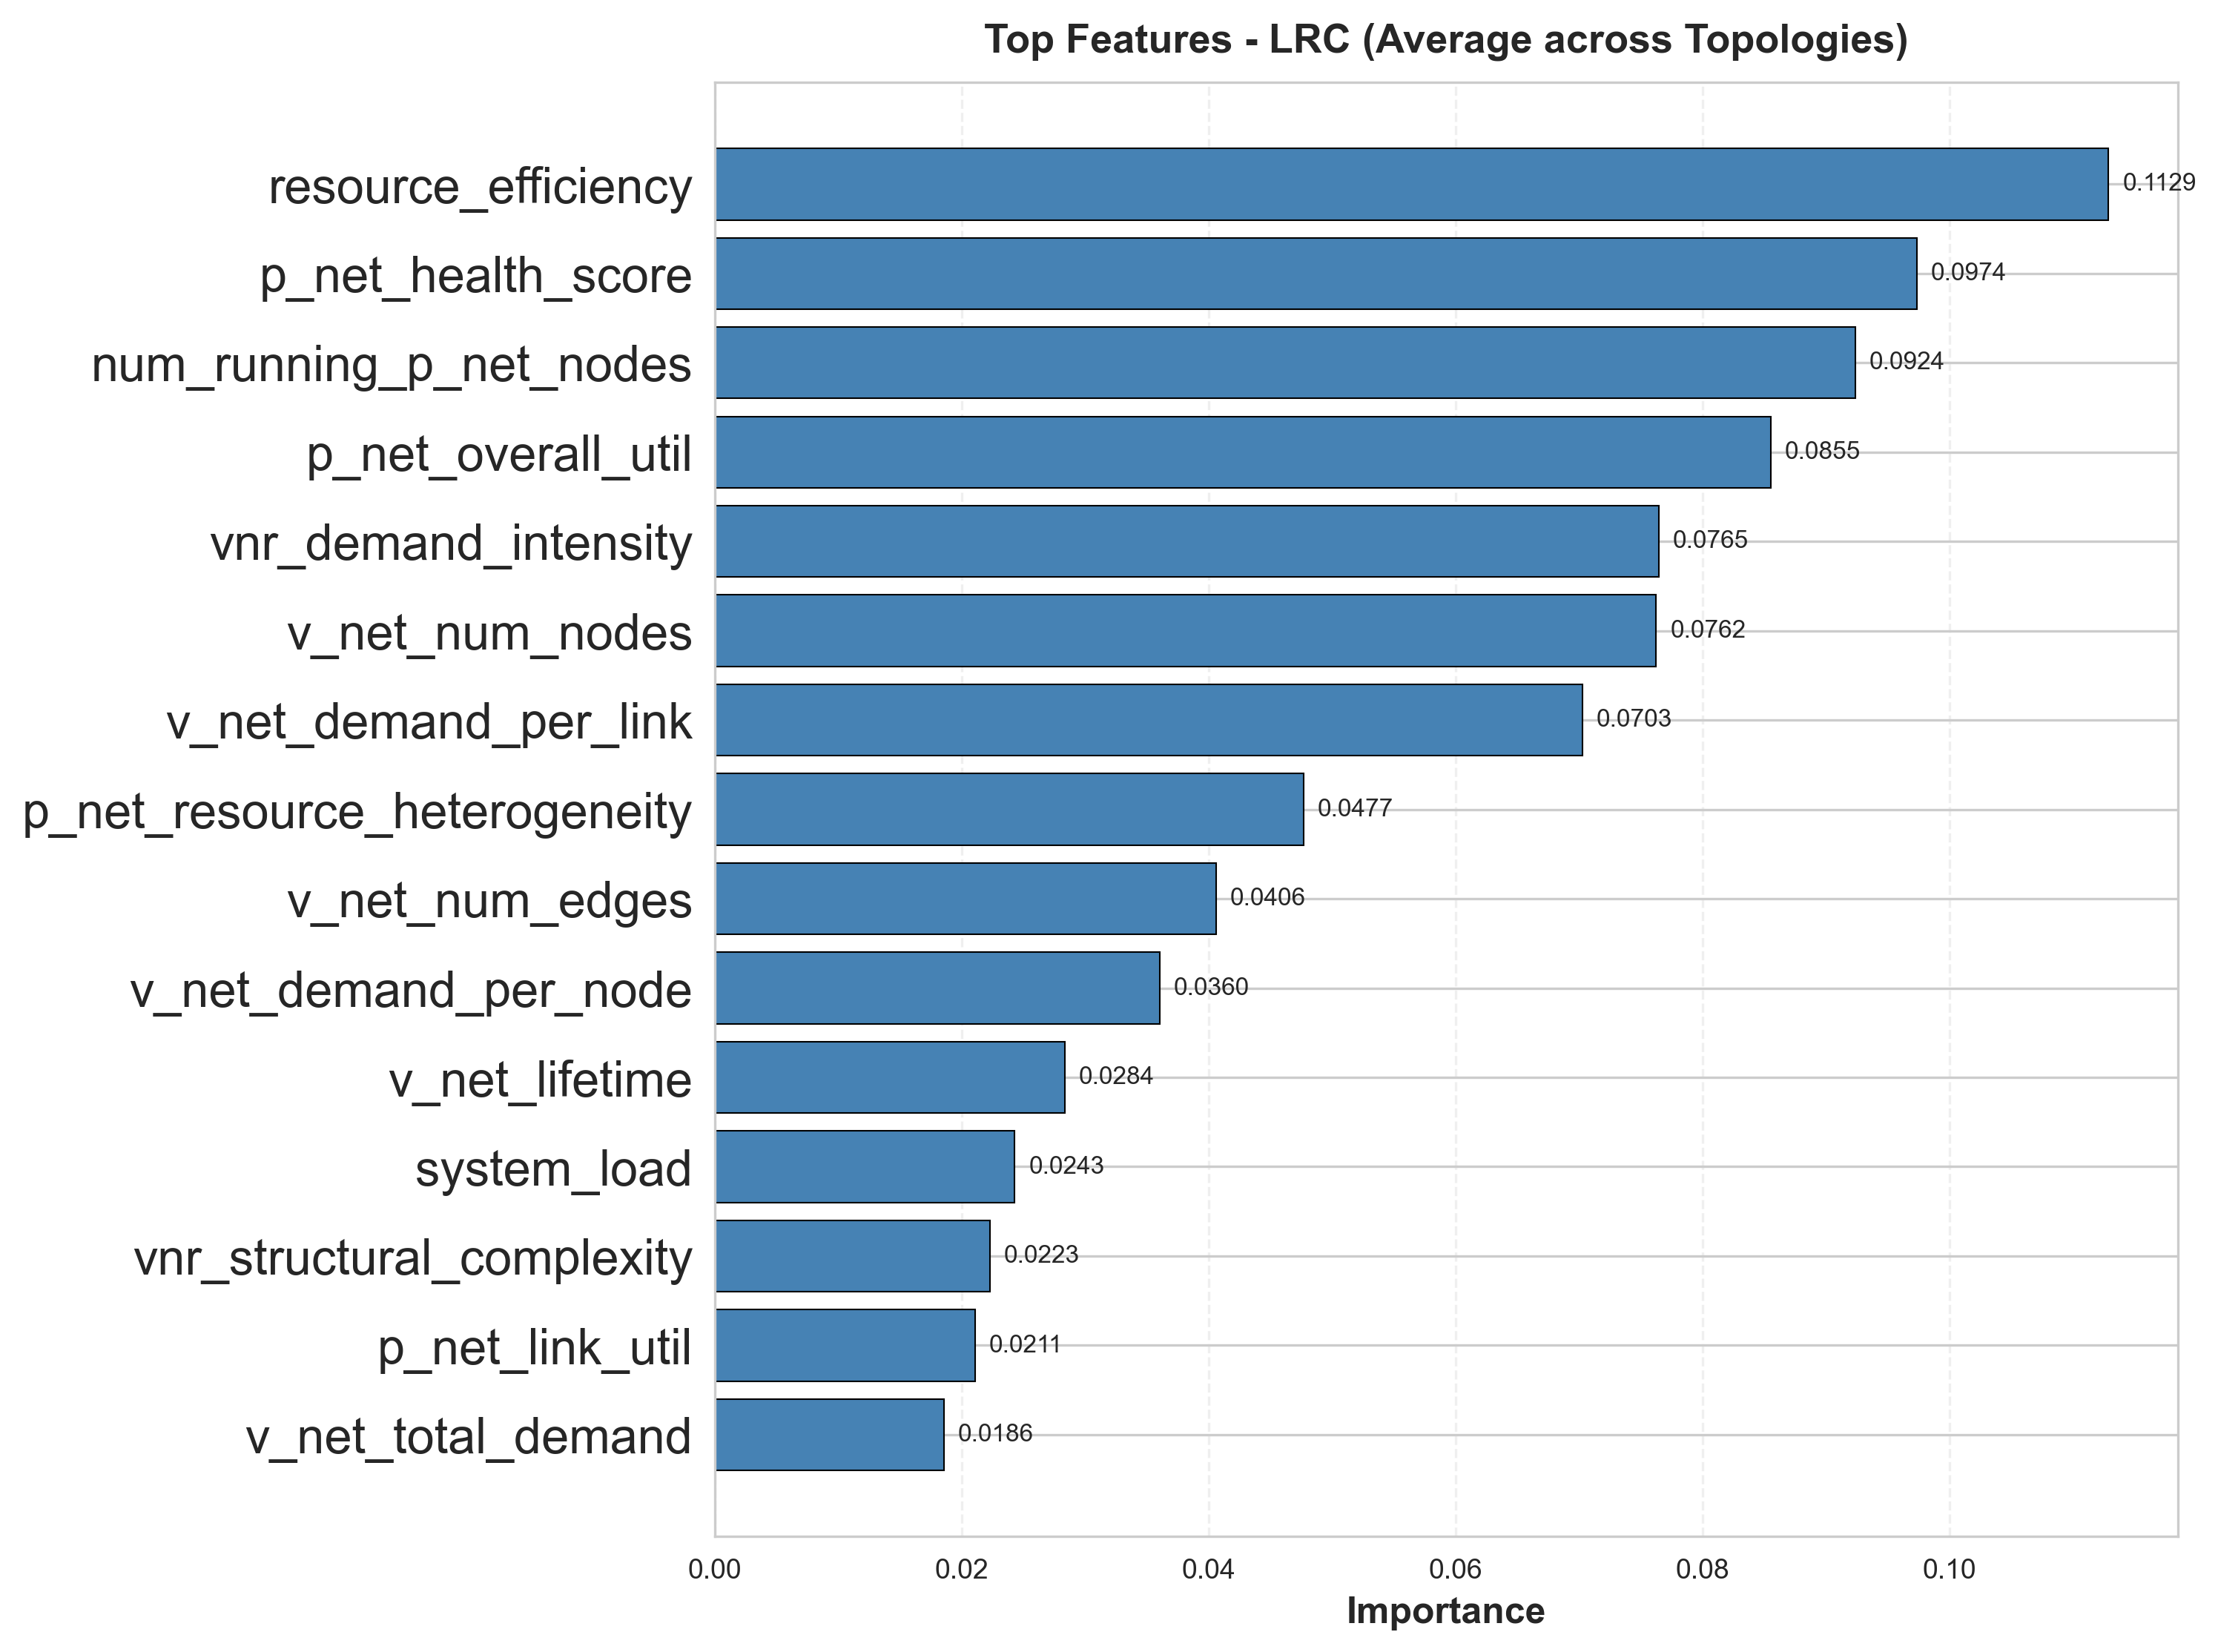
\includegraphics[width=0.95\columnwidth]{per_objective_lrc}
    \caption{Feature Importance - LRC (Long-Term Revenue-to-Cost). The top 15 most important features (average across topologies) for the LRC objective. Resource efficiency ($resource\_efficiency$) is the most critical feature with importance of 0.113, followed by physical network health score ($p\_net\_health\_score$) with 0.097.}
    \label{fig:feature-importance-lrc}
\end{figure}

\begin{figure}[H]
    \centering
    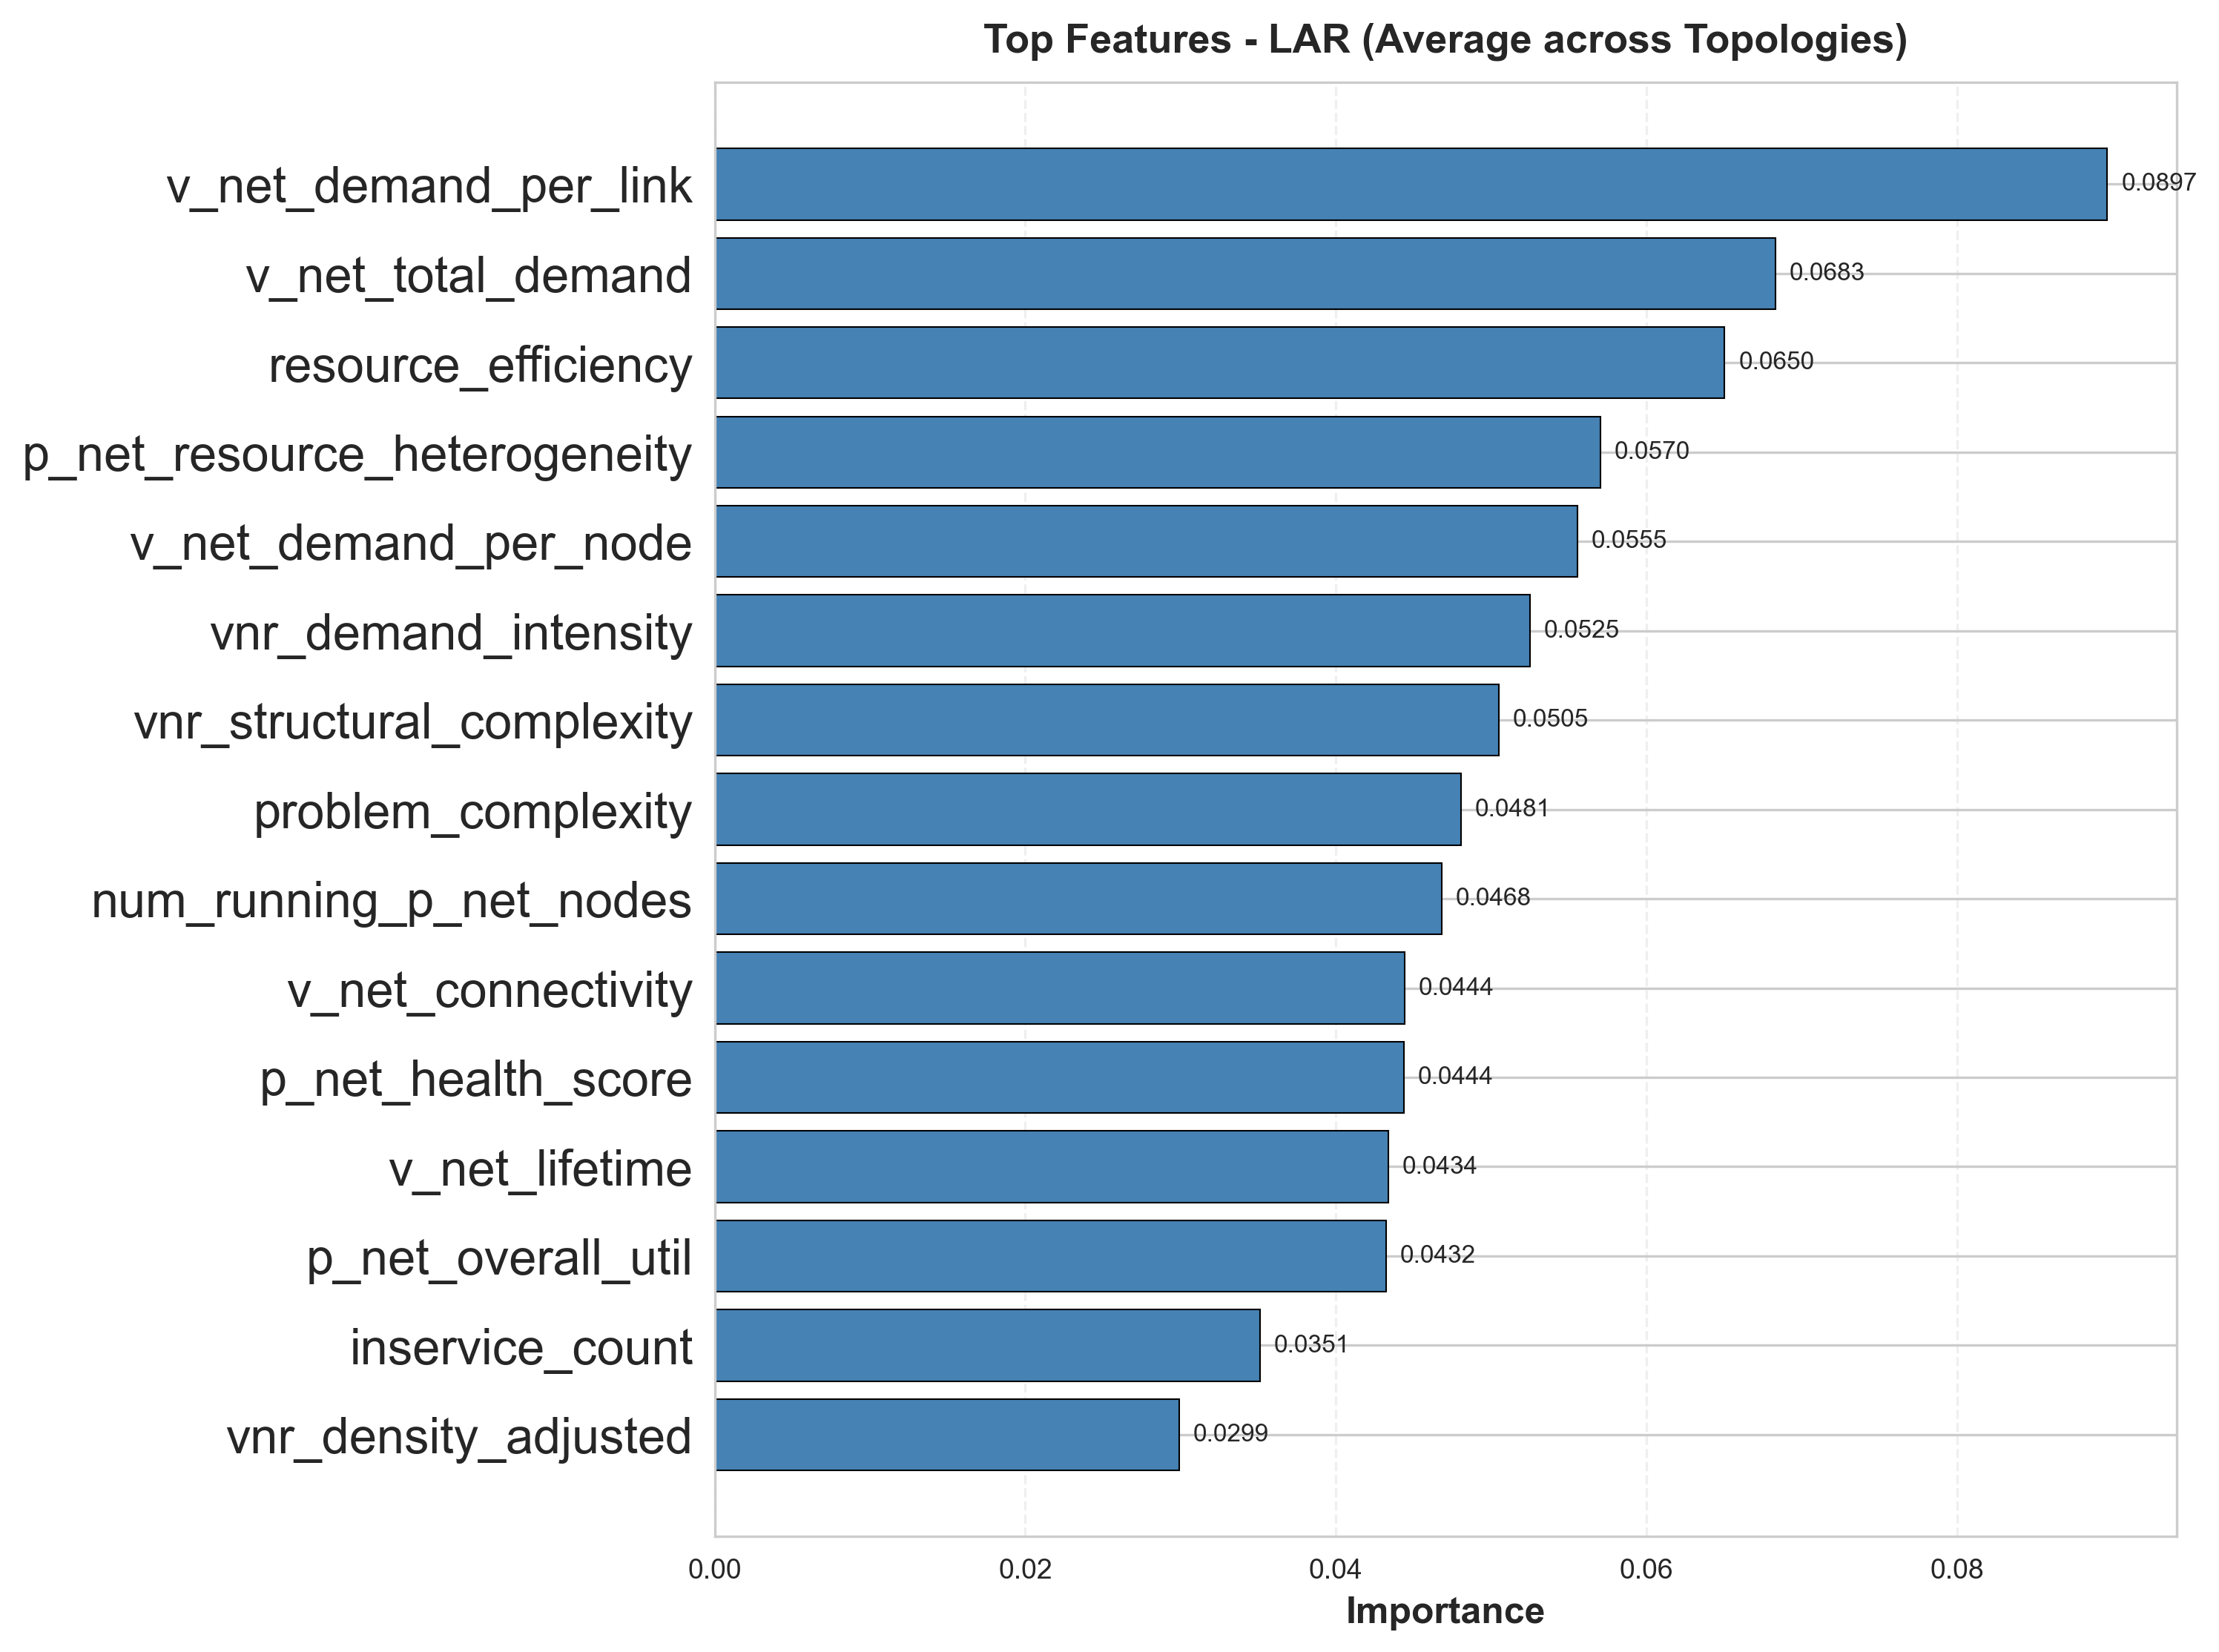
\includegraphics[width=0.95\columnwidth]{per_objective_lar}
    \caption{Feature Importance - LAR (Long-Term Average Revenue). The top 15 most important features (average across topologies) for the LAR objective. VNR link demand ($v\_net\_demand\_per\_link$) is the most important feature with 0.090, followed by total demand ($v\_net\_total\_demand$) with 0.068.}
    \label{fig:feature-importance-lar}
\end{figure}


This interpretability is critical, as it allows regulators to perform audits by verifying decisions made by the system, facilitates debugging work by enabling operators to understand system behavior, and increases confidence and acceptance of zero-touch automation.

\subsection{Inference Latency}

Prediction latency measurements for each model (based on a benchmark with 8,000 iterations):

\begin{itemize}
    \item Average time: 0.034\,ms per prediction
    \item Percentile p99: 0.055\,ms (worst case: 0.119\,ms)
    \item RL Comparison: FlagVNE requires 50-200\,ms per decision~\cite{ijcai-2024-flagvne}
\end{itemize}

Figure~\ref{fig:inference-latency-cdf} presents the cumulative distribution function (CDF) of inference latency, comparing the proposed approach with FlagVNE. The results show that more than 99\% of predictions are performed in less than 0.06\,ms, demonstrating consistency in sub-millisecond latency.

\begin{figure}[H]
\centering
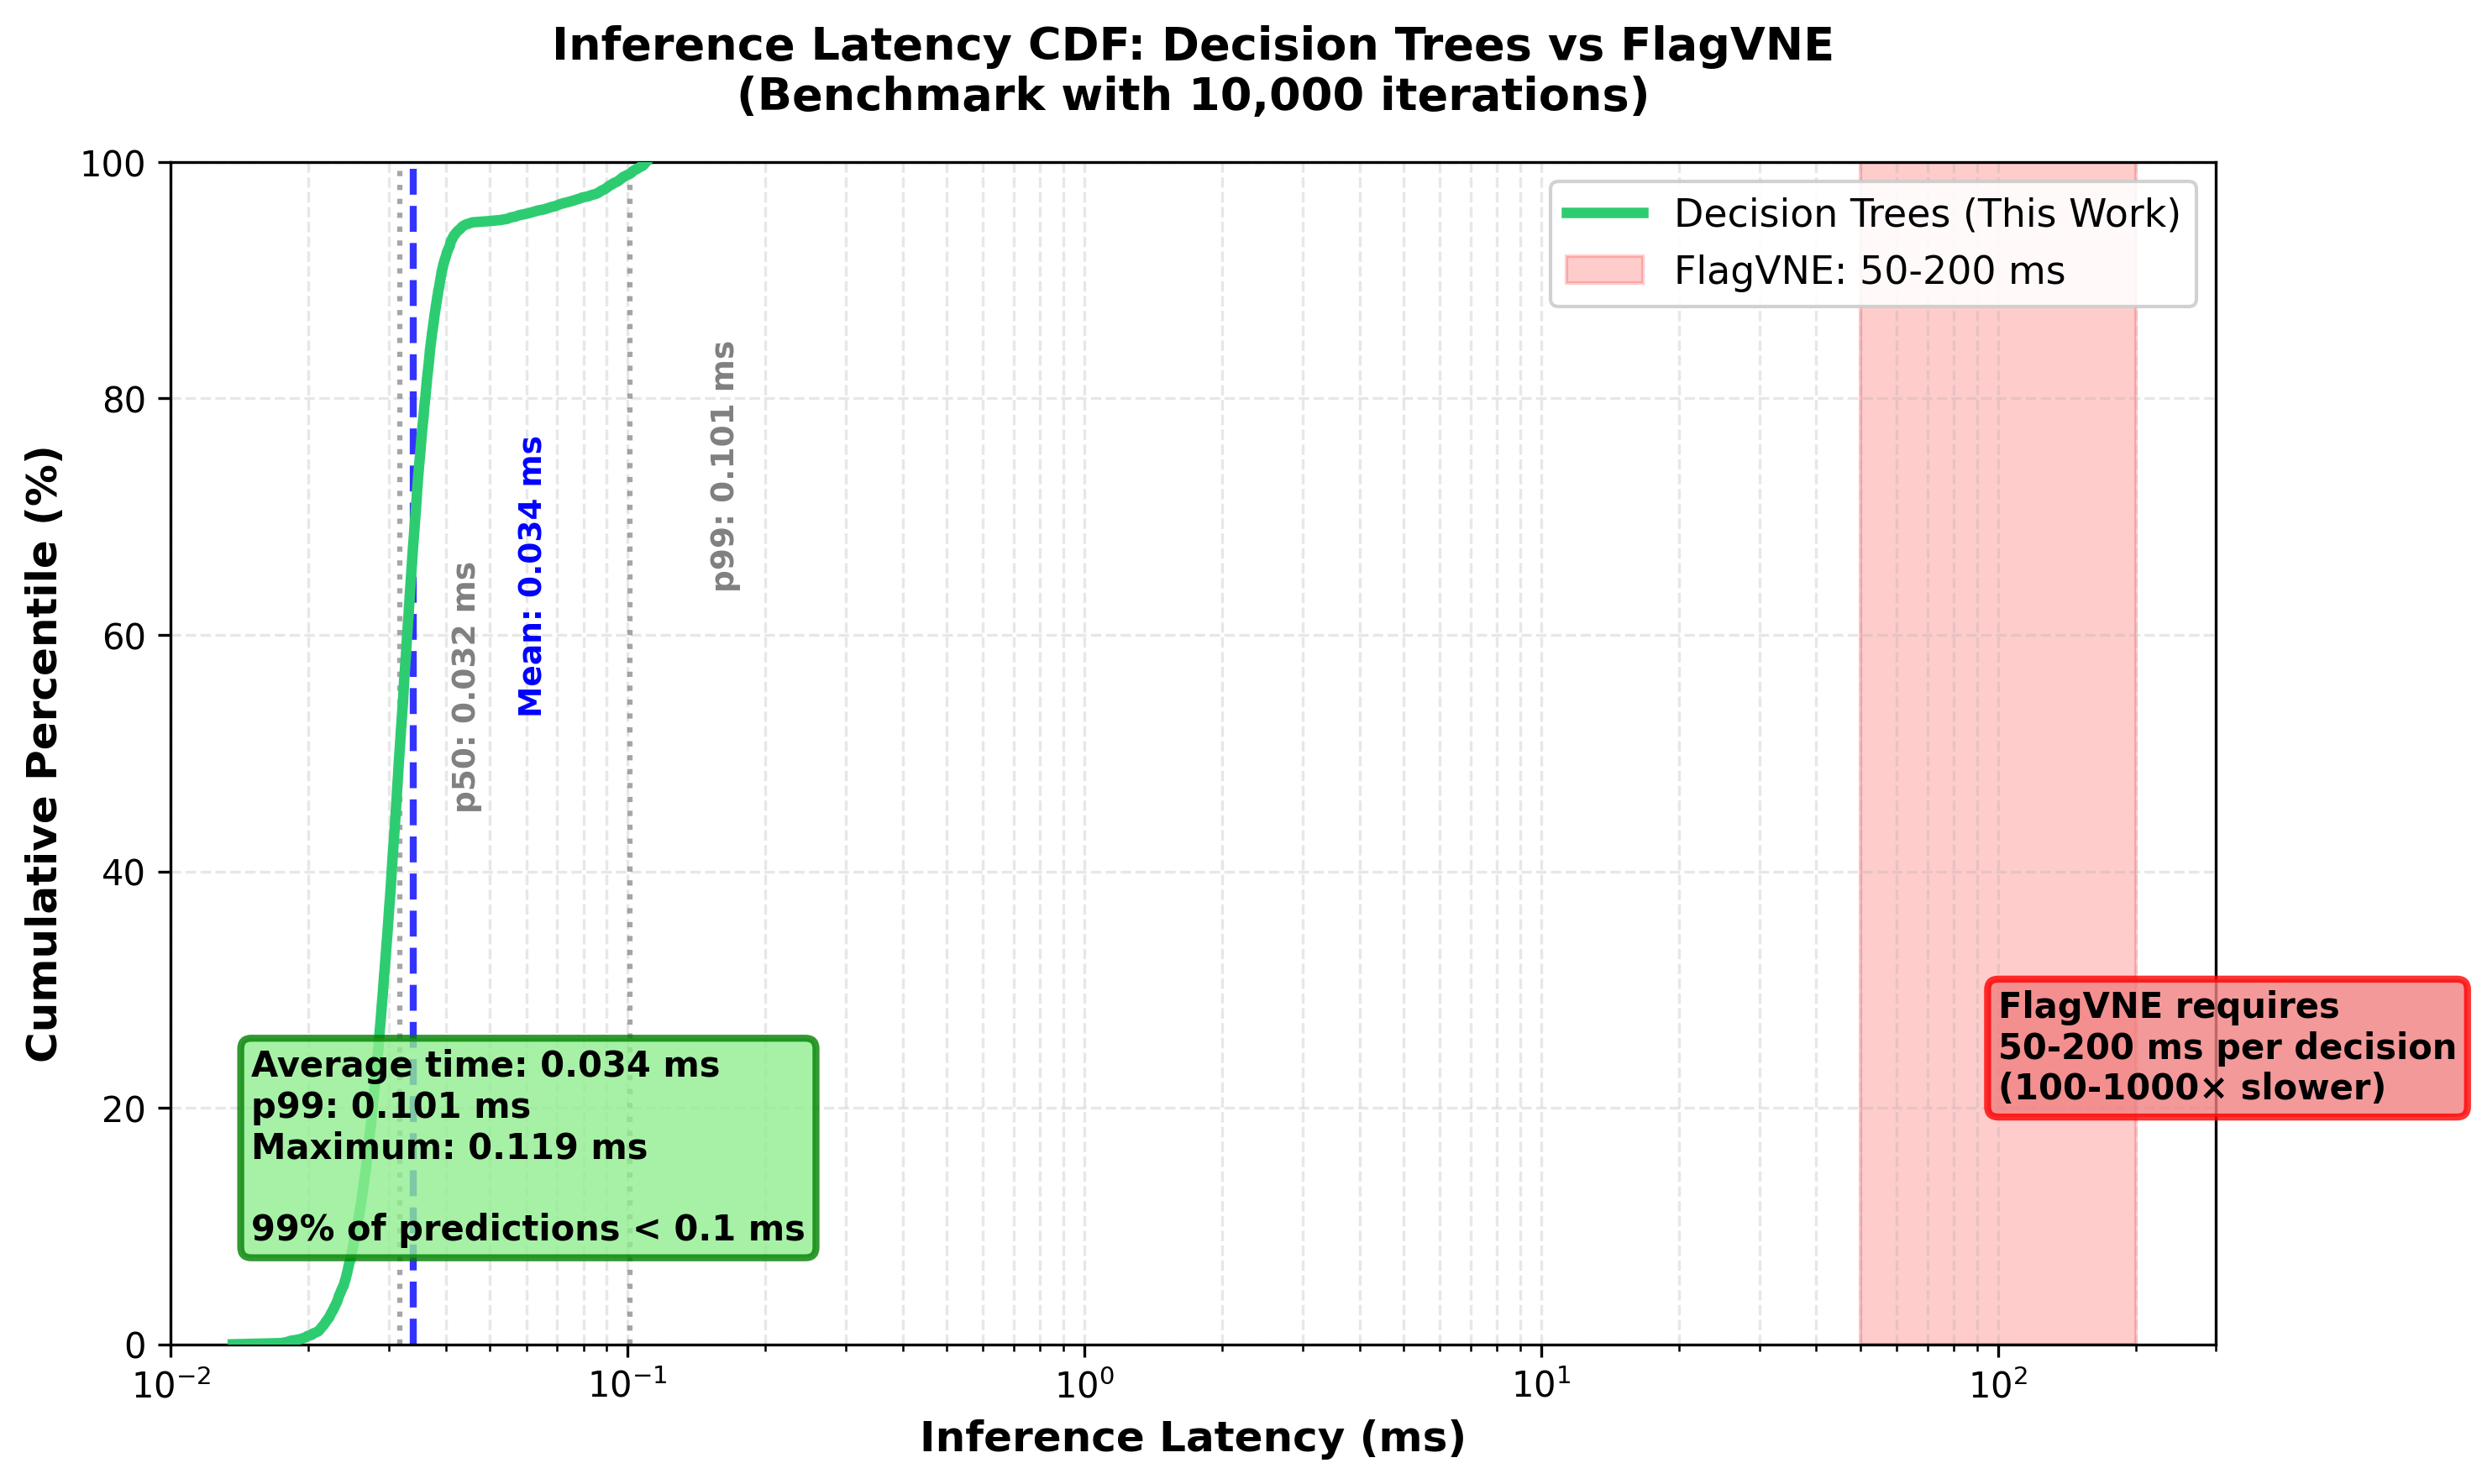
\includegraphics[width=0.95\columnwidth]{inference_latency_cdf}
\caption{Inference Latency CDF: Decision Trees vs FlagVNE. The proposed approach presents latency consistently below 0.1\,ms, while FlagVNE requires 50-200\,ms per decision (different scale on secondary axis).}
\label{fig:inference-latency-cdf}
\end{figure}

Sub-millisecond latency enables online real-time decision making, critical for zero-touch operation.

\section{Conclusion}
\label{sec:Conclusion}

The Virtual Network Embedding (VNE) problem is fundamental in modern cloud infrastructures, where mapping virtual network requests onto physical networks while optimizing multiple objectives is NP-hard. A fundamental challenge in this domain is that no single algorithm presents consistently superior performance in all scenarios, and different VNR characteristics and physical network states require distinct algorithmic approaches. Additionally, modern infrastructures demand zero-touch administration capabilities, requiring systems that can operate autonomously with interpretability and low latency for real-time decision-making.

To address this challenge, this work proposed an approach for zero-touch selection of Virtual Network Embedding algorithms using multi-objective decision trees, considering virtual network request characteristics and physical infrastructure state.
Experimental results show that the foundations of the proposed approach (decision trees, multi-objective optimization, and interpretability) are potential candidates to achieve zero-touch network control according to the ETSI ZSM standard.
The experimental analysis, based on three datacenter topologies (Tree, Fat-Tree, and Waxman-16) with 8,000 virtual network requests, showed that contextual algorithm selection can reduce processing time and improve acceptance rate in various scenarios, without requiring software updates at infrastructure endpoints.

As limitations, the model was trained on three simulated topologies, and the characteristics capture instantaneous network state.
As future work, promising directions include transfer learning between topologies, incorporation of temporal history of requests, and validation in production environments with real \textit{datacenter} workloads.

%===================================================================

\section*{\uppercase{Acknowledgements}}

Blind review.

\bibliographystyle{apalike}
{\small
\bibliography{references}}

\end{document}

